\documentclass[12pt]{article}

\usepackage[none]{hyphenat}

\usepackage{upgreek}

\usepackage{amsmath}

\usepackage{graphicx}
 
\usepackage{listings}
\usepackage{color}
 
\definecolor{codegreen}{rgb}{0,0.6,0}
\definecolor{codegray}{rgb}{0.5,0.5,0.5}
\definecolor{codepurple}{rgb}{0.58,0,0.82}
\definecolor{backcolour}{rgb}{0.95,0.95,0.92}
 
\lstdefinestyle{mystyle}{
    backgroundcolor=\color{backcolour},   
    commentstyle=\color{codegreen},
    keywordstyle=\color{magenta},
    numberstyle=\tiny\color{codegray},
    stringstyle=\color{codepurple},
    basicstyle=\footnotesize,
    breakatwhitespace=false,         
    breaklines=true,                 
    captionpos=b,                    
    keepspaces=true,                 
    numbers=left,                    
    numbersep=5pt,                  
    showspaces=false,                
    showstringspaces=false,
    showtabs=false,                  
    tabsize=2
}
 
\lstset{style=mystyle}

\usepackage{dsfont}

\usepackage{amssymb}

\def\ojoin{\setbox0=\hbox{$\bowtie$}%
  \rule[-.02ex]{.25em}{.4pt}\llap{\rule[\ht0]{.25em}{.4pt}}}
\def\leftouterjoin{\mathbin{\ojoin\mkern-5.8mu\bowtie}}
\def\rightouterjoin{\mathbin{\bowtie\mkern-5.8mu\ojoin}}
\def\fullouterjoin{\mathbin{\ojoin\mkern-5.8mu\bowtie\mkern-5.8mu\ojoin}}

\usepackage{hyperref}

\usepackage[utf8]{inputenc}

\usepackage{graphicx}
\graphicspath{ {imgs/} }

\usepackage{mathtools}

\usepackage{textcomp}

\usepackage[english]{babel}

\usepackage{tikz}

\usepackage{tcolorbox}

\usepackage{amsthm}

\setlength{\parindent}{0cm}

\renewcommand\qedsymbol{$\blacksquare$}

\usepackage{fancyhdr}
 
\pagestyle{fancy}
\fancyhf{}
\fancyhead[LE,RO]{Introduction to Databases -- Fall 2017}
\fancyhead[RE,LO]{Joshua Concon}
\fancyfoot[CE,CO]{\leftmark}
\fancyfoot[LE,RO]{\thepage}


\begin{document}

\title{CSCC43: Introduction to Databases\\ Lecture Notes}
\date{University of Toronto Scarborough -- Fall 2017}
\author{Joshua Concon}
\maketitle

Instructor is Dr. Marzieh Ahmadzadeh. Check RateMyProf. If you find any problems in these notes, feel free to contact me at conconjoshua@gmail.com. I own nothing, all copyrighted works belong to their respective owners (University of Toronto and Pearson Education).

\tableofcontents

\pagebreak

\section{Thursday, September 7, 2017}

\subsection{Definitions}

\paragraph{Data} Objects or events that could be recorded on a computer media. This includes stuff like an email, an address, a student identification number, etc.\\

However, there are two types of Data, Unstructured and Structured.

\paragraph{Structured Data} They are mostly stored in a tabular format, have types including: date, character, numeric, alphanumeric.

\paragraph{Unstructured Data} Data that must be analyzed to extract information from, does not already show information. Includes multimedia, maps, documents, pictures, voices.

\paragraph{Database} An organized collection of logically related data that can be of any size or complexity. Example:
\begin{itemize}
	\item{Student ID, name, GPA, courses taken}
	\item{Patient name, doctor's ID, ward, date of admission}
	\item{Personnel ID, base salary, bonus, hours of work}
\end{itemize}

\underline{Another Example:}

\begin{center}
 \begin{tabular}{||c c c||} 
 \hline
 ID & Course & Mark \\ [0.5ex] 
 \hline\hline
 100 & CSCC43 & A \\ 
 \hline
 100 & CSCC44 & B \\
 \hline
 100 & CSCC52 & A+  \\
 \hline
 200 & CSCC43 & A+\\
 \hline
 200 & CSCC62 & B\\ [1ex] 
 \hline
\end{tabular}
\end{center}

\paragraph{Database Management System (DBMS)} A software that sits between users and databases, responsibilities include:
\begin{itemize}
	\item{Allowing users to create, update, sort or retrieve data}
	\item{Enforcing the integrity of data (consistency, etc.)}
	\item{Improving performance when dealing with huge data or many queries}
	\item{Assuring the durability of the data}
	\item{Allowing data to be shared among different programs}
	\item{managing concurrent access by multiple users/processes}
\end{itemize}

\paragraph{Information} Information is data that has been process in order to increase user knowledge, could be data provided in a way that can be analyzed easily (i.e. has labels, maybe graphs showing relationships, etc.)

\paragraph{Metadata} "Data about data". Data that describes the properties of end-user data and it's context, it helps the database designer understand what kind of data exists and what it means. Examples include name, type, length, allowable values, ownership (stewardship), source...
\\
\underline{Example:}\\
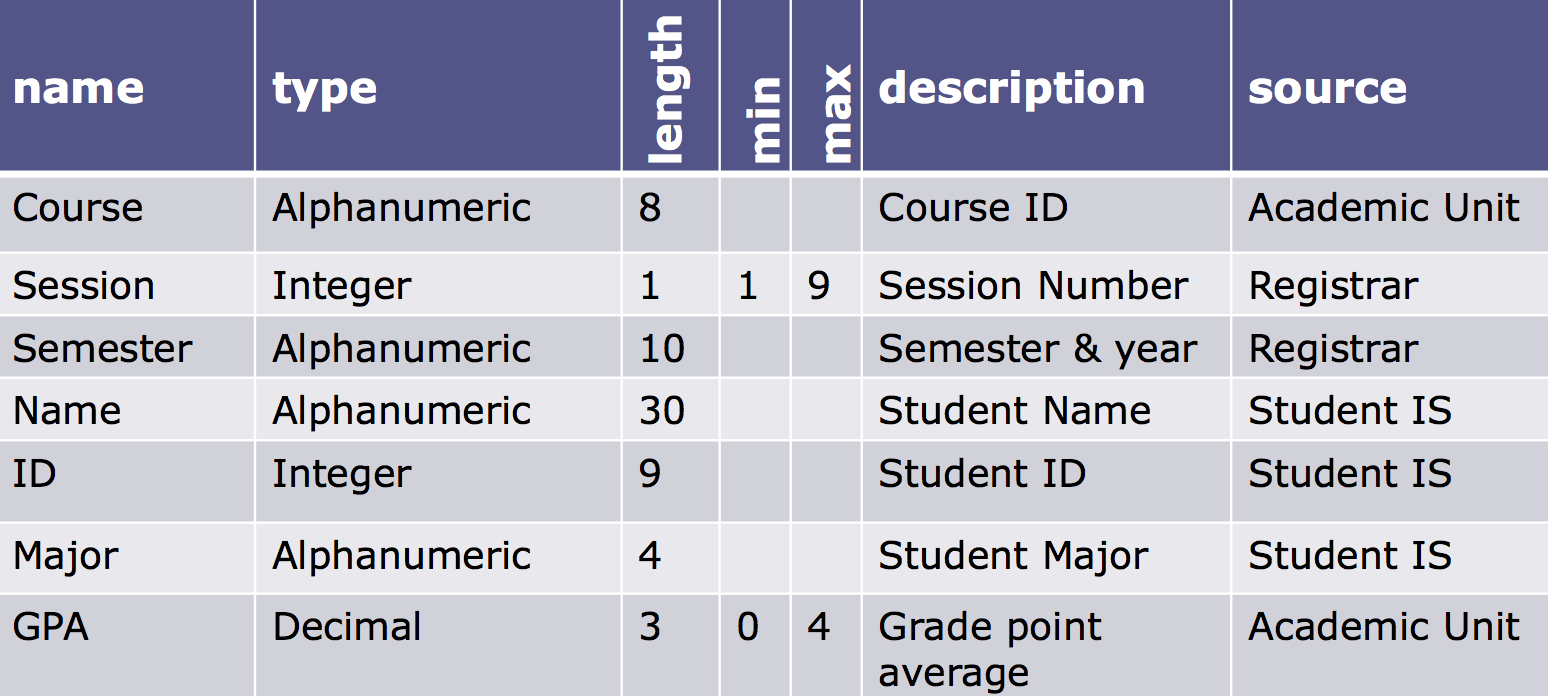
\includegraphics[scale=0.5]{lec1-1}

\subsection{How do we store data?}

There are two ways we can store data, either the Traditional file system or the database approach.

\subsubsection{Traditional File System}

The Traditional File System includes files that are also collections of related data, was used prior to the invention of databases, but has its own disadvantages.\\
\\
\underline{Example of a file system:}\\
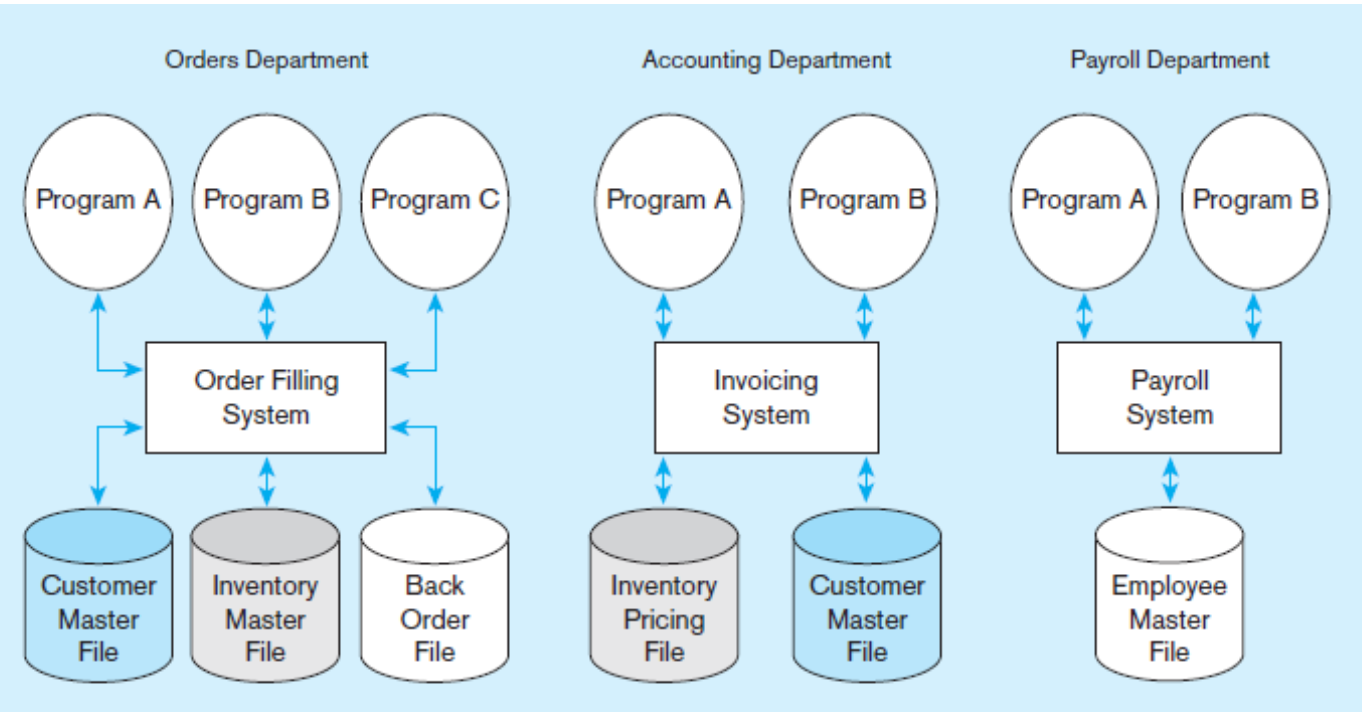
\includegraphics[scale=0.5]{lec1-2}\\

\underline{Disadvantages:}
\paragraph{Program-Data Dependence} If the data is changes, all programs that used the data should be altered to. To use an example from the previous image, if the length of data such as customer name is changed, order filling system programs and invoice system programs are both affected. Using the database approach, this is managed by a Database Management System and no change in order filling or account programs are required, only on the file itself.

\paragraph{Duplication of Data} As seen from the last image, the order filling system and the invoice system both have a customer master file. This is a waste of space as it is essentially two sets of the same data, and reliable metadata is difficult to establish since it may be inconsistent. Changes to one copy must also be applied to the other, so this may compromises the files' data integrity.

\paragraph{Limited Data Sharing} Since each application has its own data, data sharing between applications is not easy, a system does not have access to another system's data. With the database approach, data sharing is doable.

\paragraph{Length Development Times} Each new application should be started from scratch by designing a new file format and description, however, in the database approach, you only need to design your database once, and can easily access the data you need.

\paragraph{Excessive Program Maintenance} All preceding factors creates heavy program maintenance, so to avoid these disadvantages, the database approach is preferred. Note that if a database is not properly designed, mentioned disadvantages may not disappear.

\subsubsection{Database Approach}

The database approach creates a repository of shared data, data is managed by a controlling agent (Database Management System), and all data is stored in a standardized convenient form.\\
\\
\underline{Visualization Example:}\\
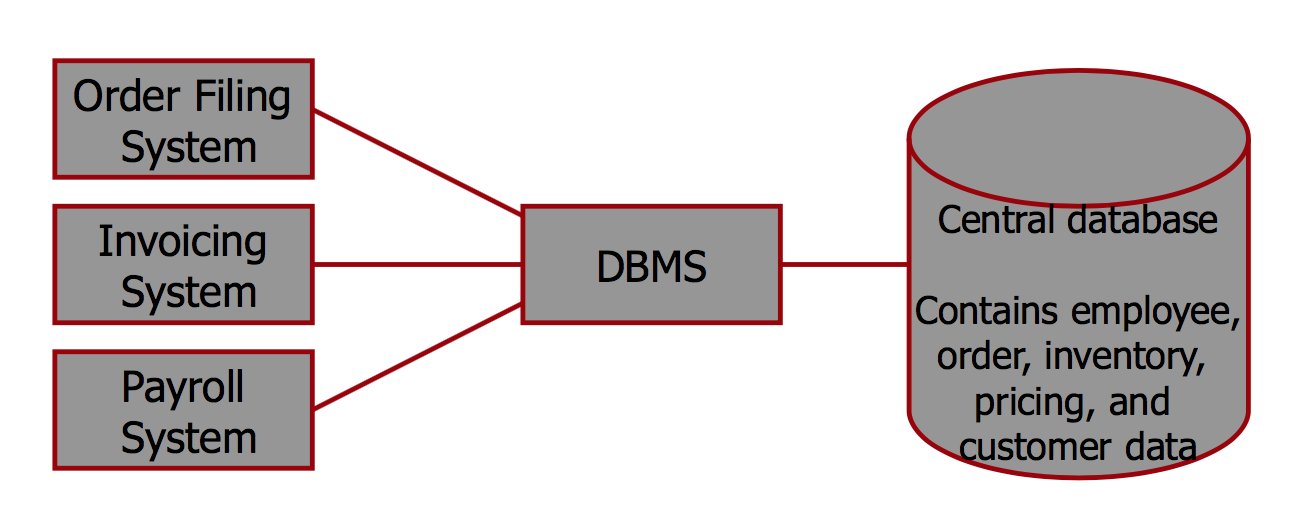
\includegraphics[scale=0.5]{lec1-3}\\

Every Database uses a data model, and this data model is a notation for describing data that specifies the structure of the data, the constrains on the content of the data, and the operations on the data.\\
\\
Some examples of data models include a relational data model, a semistructured data model, unstructured data, and an Object-oriented model.

\subsection{Relational Data Model}

The main concept of the relational data model is a relation, which is based off the concept of relations in math. A relation in a database is like a table consisting of rows and columns.\\
\\
\underline{Example:}\\
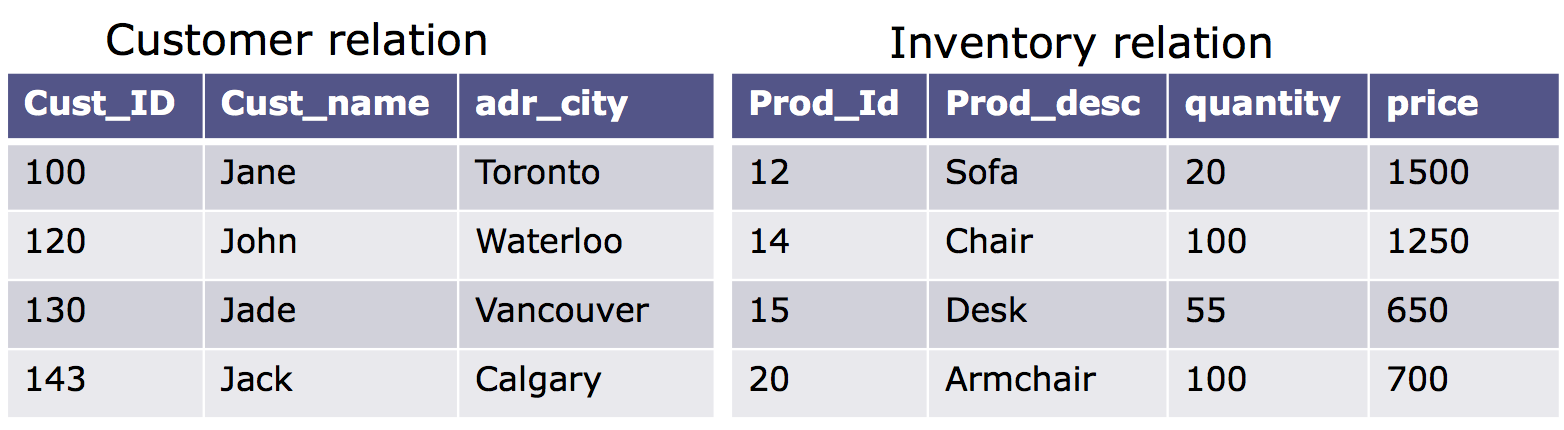
\includegraphics[scale=0.5]{lec1-4}\\

\subsubsection{Advantages}

\paragraph{Program-data independence} Metadata is stored in a central location called a repository, and data could be changed independent of what program uses it.

\paragraph{Planned data redundancy} Data is only duplicated when we want it to be duplicated, so we can control redundancy.

\paragraph{Improved data consistency} Which is implied since data redundancy is eliminated.

\paragraph{Increased productivity of application development} Since the application does not deal with the data management, since it is taken care of by the Database Management System, so time and cost of development is saved.

\paragraph{Enforcement of standards} Standards are enforced by the uniform procedures for accessing and updating data.

\paragraph{Improved data quality} By defining constraints that the data must follow.

\paragraph{Improved data accessibility and responsiveness} Can be done by using a query system to access data.

\paragraph{Reduced program maintenance} Because of data-program independence, changing the data does not affect any program.

\paragraph{Improved data sharing} By creating a user view and since all applications share the same data already, data sharing is doable.

\subsubsection{Cost and Risk}

\paragraph{New specialized personnel} Companies need to hire new people for database design and database administration services.

\paragraph{Installation and Management of Cost and Complexity} Implementation of the database and scaling it will be a new concern for companies

\paragraph{Conversion Costs} Costs for converting legacy system to a modern database

\paragraph{Need for backup and recovery} New costs and concerns for backing up the database and new services companies must worry about for recovery.

\paragraph{Organizational Conflict} On data definition, data format and right to update data.

\subsection{Database Development Process}

\paragraph{Model the rule of the organization} Such as, "each student at UofT can take up to 5 courses in one semester"

\paragraph{Explore a relation between various entities} Such as, "A course might be taken by many students", "A student must take at least one course", etc.

\paragraph{Create your relation} Creating the tables with relations between the entities and data associated with each object

\paragraph{Normalize your relation} We will learn what this is later in the course

\paragraph{Implementation} Actual Implementation of the database

\newpage

\section{Thursday, September 14, 2017}

\subsection{Relational Data Model}

A relational data model has 3 components, one of which is an \textbf{Entity}, which contains the Entity itself: which is a concept that we maintain data about, an \textbf{Entity Type}: which corresponds to a table and what the information in the table refers to, and an \textbf{Entity Instance}, which is an instance of an entity, such as (100, Jane, 3.5), which refers to a student named Jane with a Student ID of 100 and a cGPA of 3.5.\\

The notation for the entities is as follows (It's mostly just a rectangle tbh):\\
\\
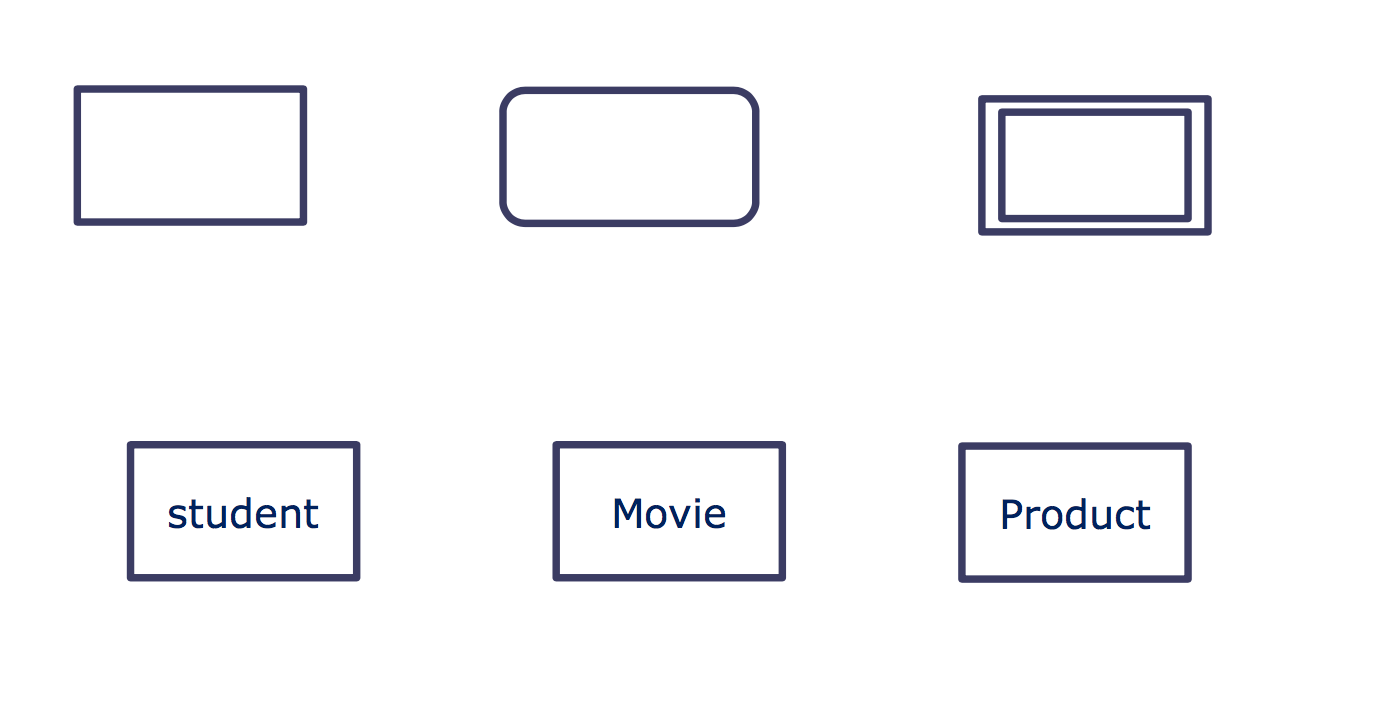
\includegraphics[scale=0.5]{lec2-1}


Another one of the 3 components is a \textbf{Relationship}, which contains a \textbf{Relationship Instance}: which is an association between entity instances itself, such as a Student named Jane taking 3 courses (which is a 1:M relationship as 1 student can take many courses) and a \textbf{Relationship Type}: which was the type of relationship, such as (1:M) as described in the previous example.\\
\\
The notation for relationship types is as follows:\\
\\
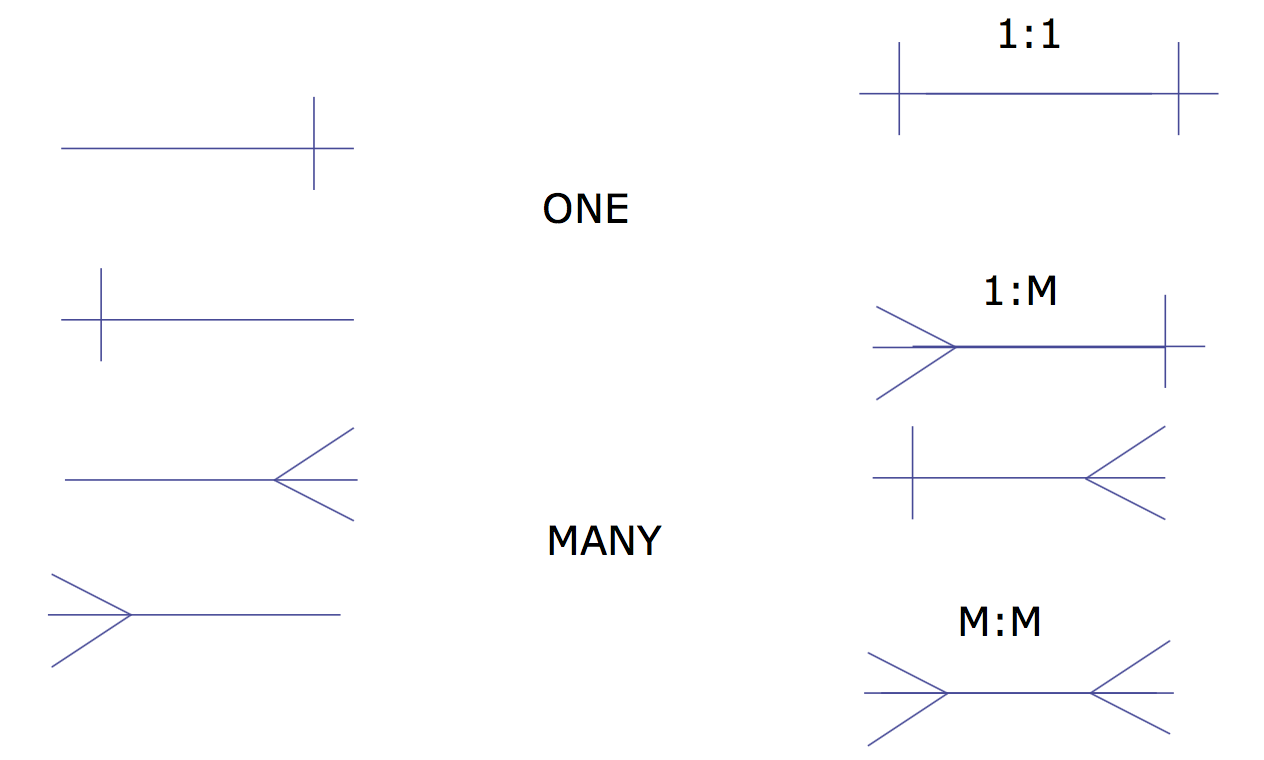
\includegraphics[scale=0.5]{lec2-2}

The last of the 3 components are \textbf{attributes}, which are properties or characteristics of an entity, which often corresponds to a field in a table. For example, for a student entity, an example attribute for this student entity would be "cgpa" or "student ID".

\subsection{Database Analysis}

Before the database can be created, you must first gather user requirements for the data, what exactly we need this data to do and what kind of constraints we need. We'll need to know the entities we would have to make for the database and what relationships these entities have with each other.\\
\\
Afterwards, we must develop a data model, more specifically, an Entity Relationship (ER) model.

\subsection{Business Rules}

Business Rules are statements that define or constrain some aspect of the business. For Example: "at UofT, a student must take at least one course in each semester." These statements are usually derived from policies, procedures, events, and functions, for example: "at UofT, a student should have passed the prerequisites to be able to take a course." These constraints and definitions must also be familiar to the end users and must be automatically enforced by the Database Management Software.\\
\\
We gather these business rules by speaking to people involved in the business that this database is being created for and by investigating business documents.

\subsubsection{Cardinality Constraints}

\textbf{Cardinality Constraints} are rules that specifies the number of instances of one entity that can be associated with each instance of another entity. Examples include:
\begin{itemize}
	\item{"Each student at UofT can take \underline{at most 5} courses each semester"}
	\item{"Each person can have \underline{at most 1} family doctor"}
	\item{"A movie can be screened \underline{at most 6} times a day"}
\end{itemize}

\textbf{Minimum Cardinality} is the minimum number of instances of one entity that can be related to the other instance.\\
\\
\textbf{Maximum Cardinality} is the maximum number of instances of one entity that may be related to each instance of another entity.\\
\\
The notation for these cardinality constraints are as such:\\
\\
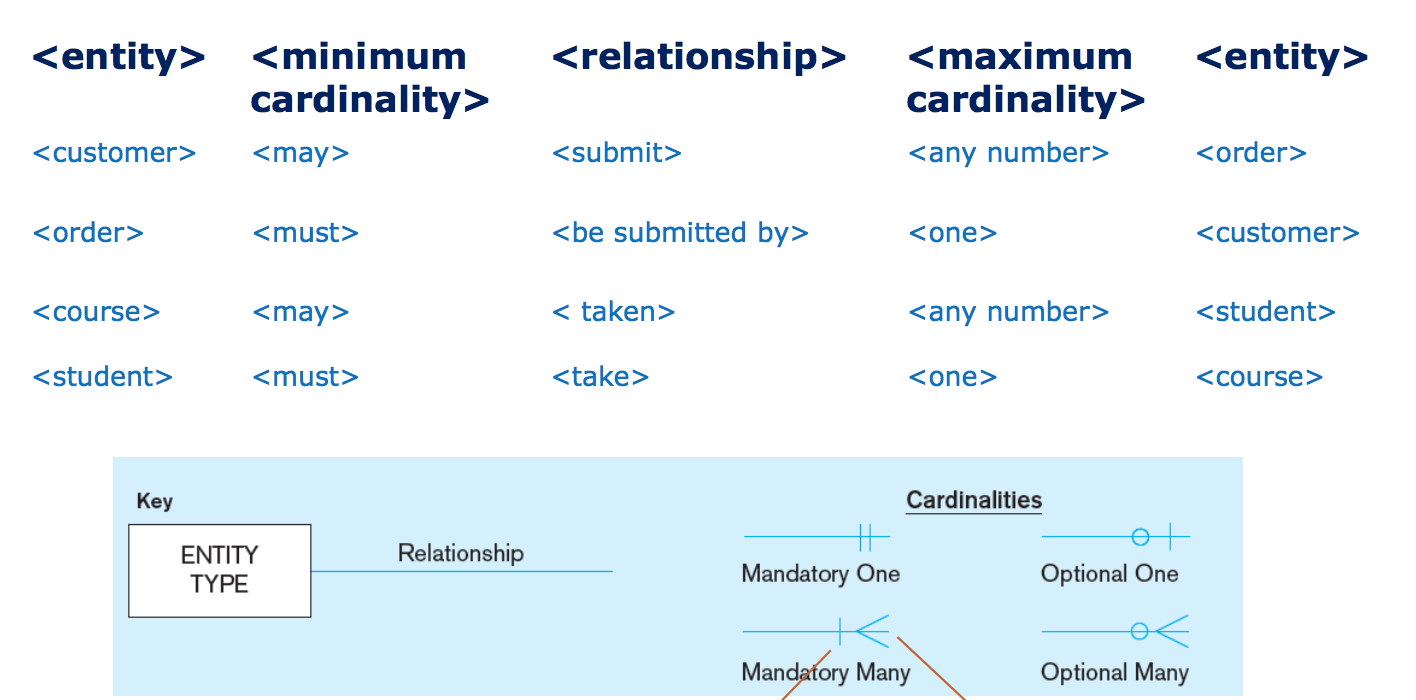
\includegraphics[scale=0.5]{lec2-3}

\subsection{Entity Relationship (ER) Model}

After business rules have been collected, from these rules, relationships between entities can be modelled, and for this, we will use the Entity Relationship Model. This model is a logical representation of the data for an organization, the entities are to represent the data, and the relationships are to show the associations between entities.

\subsubsection{Entity}

An entity is the building block of the Entity Relationship Model, such examples include:
\begin{itemize}
	\item{Person: \textit{employee, student, patient}}
	\item{Place: \textit{store, warehouse, state, drugstore}}
	\item{Object: \textit{machine, building, automobile}}
\end{itemize}

An entity is supposed to have a noun name and is meant to be general.\\
\\
Each entity usually consists of several \textbf{attributes.}\\
\\
An entity should be an object that will have many instances in the database, and object that will be composed of multiple attributes, and/or an object that we are trying to model. However, it should also not be a user of the database system or an output of the database system.

\subsubsection{The Weak shall fear the Strong}

There are two different types of Entities, \textbf{Strong} and \textbf{Weak} entities.\\
\\
\underline{Strong entities} exist independently of other types of entities and have their own unique identifier (e.g students, employee, course, surgeon, independent black woman who need no man).\\
\\
\underline{Weak entities} depend on a strong entity, which may or may not be their identifying owner, and cannot exist on it's own. They also do not have a unique identifier, only a partial identifier, and the entity box and partial identifier have double lines.\\
\\
The following is an example of a weak entity:\\
\\
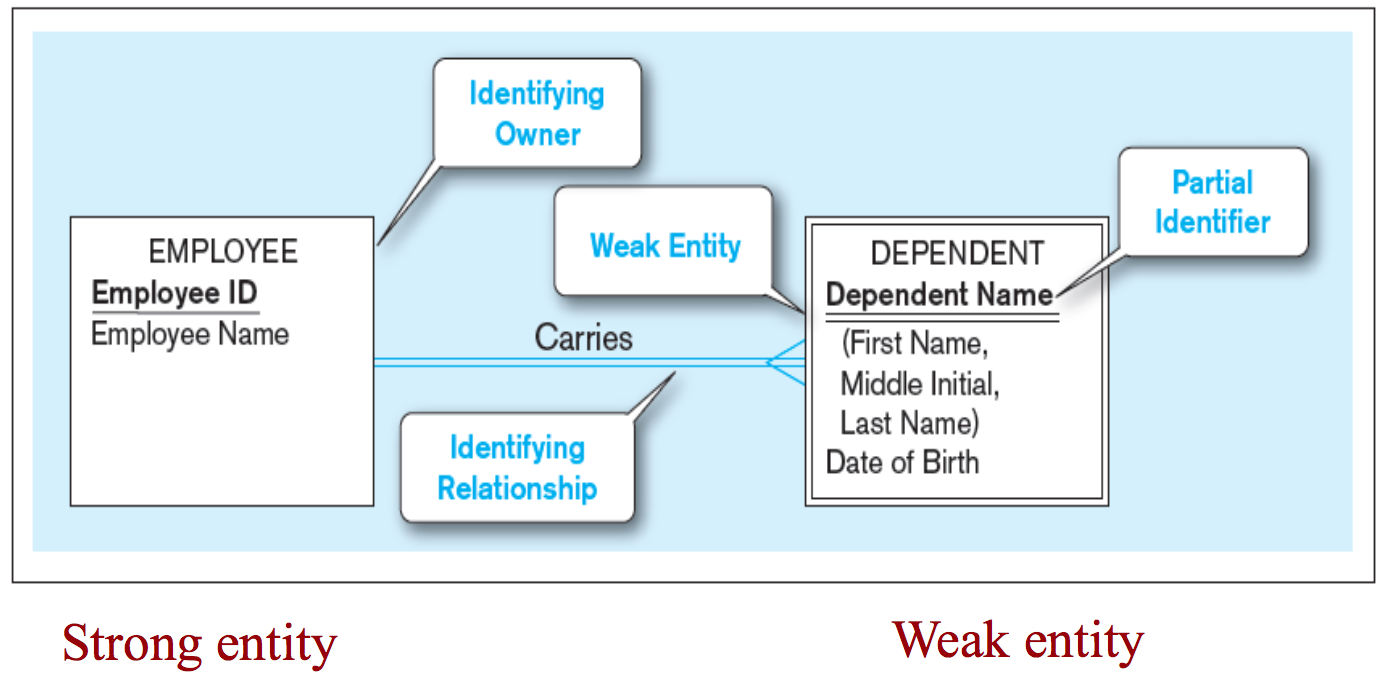
\includegraphics[scale=0.5]{lec2-4}

\subsubsection{Attributes}

Each entity type has a set of \textbf{attributes} associated with it, and by default, the name of an attribute starts with a capital.\\
\\
An attribute has different types, including: required, optional, simple, composite, single values, multivalued, stored, derived, and identifier.
\paragraph{Required Attributes} Required Attributes should have a value. Must be boldfaced or represented by a special character in E-R Diagrams.

\paragraph{Optional Attributes} Optional Attributes can be null. May be represented by an 'o' in E-R Diagrams.

\paragraph{Composite Attributes} An attribute that has meaningful component parts. For example: an address can be broken down to city, street, etc. It is up to the user as how to define these attributes. If you might use only part of an attribute, you might want to separate it as its own attribute.

\paragraph{Simple Attributes} An attribute that cannot be broken down into smaller components, such as a StudentID.

\paragraph{Multivalued Attributes} An attribute that can have more that one value. For example, skill can be 'programmer', 'analyst', etc. This type of attribute is represented with curly braces {} in ER diagrams.

\paragraph{Single Valued Attributes} An attribute that can only have one value, such as an attribute that can only be a boolean (True or False).

\paragraph{Derived Attributes} An attribute that is derived from other stored attributes. For example, years employed can be derived from today's date minus date employed. This type of attribute is represented with square brackets [] in ER diagrams.

\paragraph{Stored Attributes} An attribute that is not derived from other stored attributes, and is just stored.

\paragraph{Identifier Attributes} An attribute whose value distinguishes instances of an entity type, so no two instances are referred to by one identifier, such as an EmployeeID for example.

\paragraph{Composite Identifier} An identifier that consists of a composite attribute.

For naming these attributes, it should be a unique singular noun or noun phrase such as 'Customer ID' or 'Product Minimum Price'. The name should also follow a standard for uniqueness, such as [Entity type name { [ Qualifier ] }] Class, where the Qualifier is a phrase to constrain the class, and the Class is the properties of the entities. An example of an attribute under this template is 'Customer hourly wage'. Similar attributes of different entity types should use the same qualifiers and classes, such as 'Faculty Residence City' and 'Student Residence City'.

\subsubsection{Criteria for Identifiers}

Identifiers must be values that will never be null and will not change in value. It is ideal to substitute new, simple keys for long, composite keys if possible.

\subsubsection{Modelling Relationships}

A relationship in E-R diagrams are modelled by verbs and is represented by a line labelled with the name of the relationship.

\paragraph{Degree of Relationships} The degree of a relationship is the number of entity types  that participate in it, so for example, a \textbf{Unary} relationship would refer to one entity related to another of the same type, a \textbf{Binary} relationship would refer to two different entities, a \textbf{Ternary} relationship would refer to three different entity types.

\newpage

\section{Thursday, September 21, 2017}

\subsection{Associative Entity}

When you have a many to many relationship, and that relationship requires to have attributes assigned to it, you can create an associative entity.\\
\\
\underline{Example:}\\
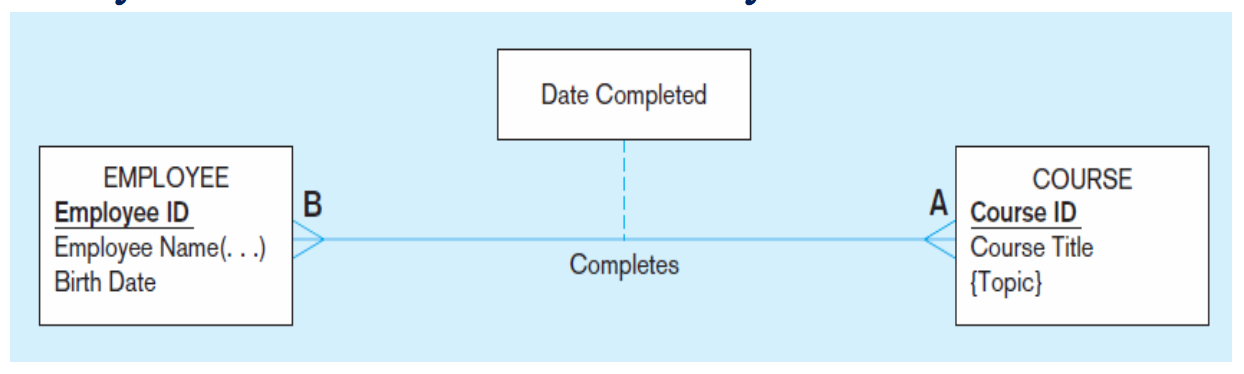
\includegraphics[scale=0.5]{lec3-1}

To denote an associative entity, you use a rounded box for the attributes, you define an identifier, and for a Many to Many relationship between entities $A$ and $B$, define the associative entity as $C$ and relate the entities as such $A:C$, as one to many and $B:C$ as one to many as well.\\
\\
\begin{tcolorbox}
	Note that Many to Many relationships cannot be implemented using a relational database.
\end{tcolorbox}

\subsection{Multiple Relationships}

It is possible that one entity can participate in more than one relationship. The relationship could be in any degree or cardinality (Mandatory or optional, any combination of 1 or many to 1 or many).\\
\\
\underline{Example:}\\
In $X$ Company, Sue manages 2 departments (finances and sale) in which 10 and 5 people work respectively. Mike manages human resource department in which 3 people are working. He is also responsible for managing project $A$ in this organization.\\
\\
The ER diagram looks like the following:\\
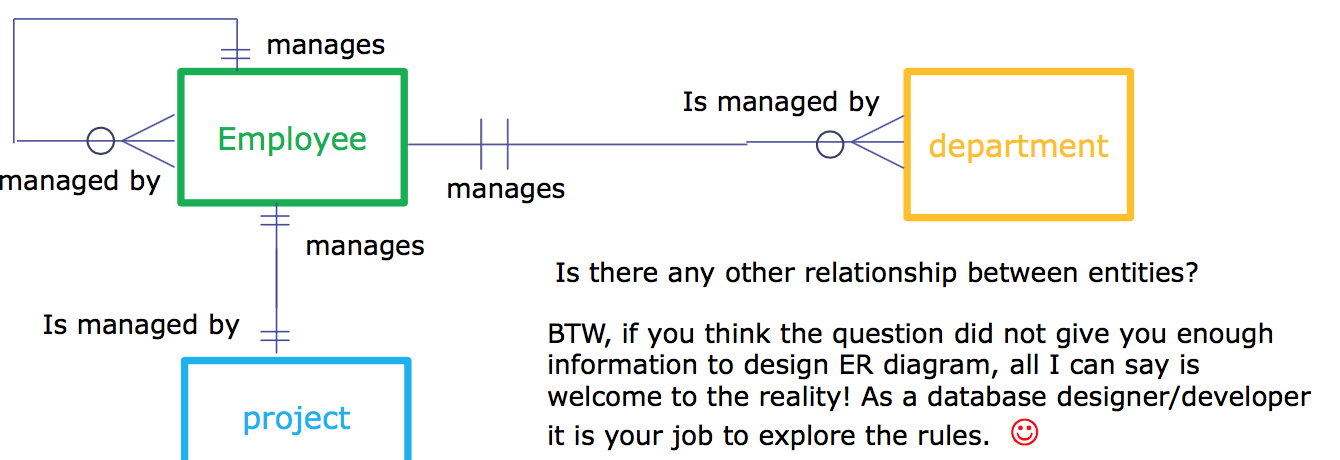
\includegraphics[scale=0.5]{lec3-2}

\subsection{Representing Multivalued Attribute}

It's generally not a good idea to have a multivalued attribute, as it can be represented as an attribute or an entity, and if it is represented by an entity, identifiers are needed for that entity. As an entity, it will result in a one to many relationship.

\subsection{Time -- Dependent Data}

Some data change their value over time and you may need to keep the history of this change. We would need to keep track of \textbf{Time stamps}, time values that is associated with a data value, often indicating when some event occurred that affected the data value.

\subsection{Enhanced ER diagram (EER)}

The ER model has been suitable for modelling most common business problems, but as business relationships get more complex, business data get more complex as well, so we would need a more complex tool to represent our model, such as an EER.\\
\\
An EER model is a model that has resulted from extending the original Entity Relationship model with new modelling constructs. The most important modelling construct incorporated in the EER model is the supertype/subtype relationships. The ideas of supertypes, subtypes and inheritance are the same parent-child concepts in object oriented software design. The only difference is that in object oriented programming, there is also the concept of behaviour, but in EER, the entities only inherit attributes.

\subsubsection{Attribute Inheritance}

Subtype entities inherit values of all attributes of the supertype, and an instance of a subtype is also an instance of a supertype.\\
\\
\underline{Examples:}\\
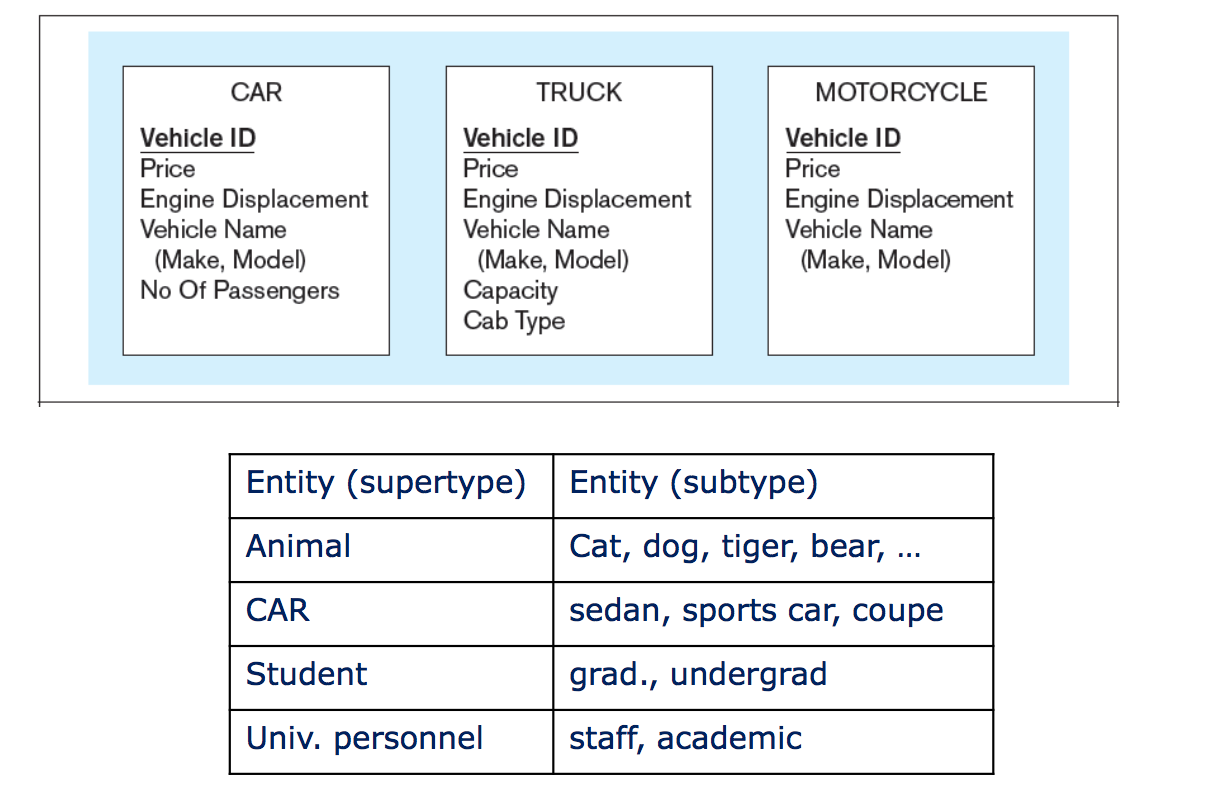
\includegraphics[scale=0.5]{lec3-3}\\
\\
and notation is as follows:\\
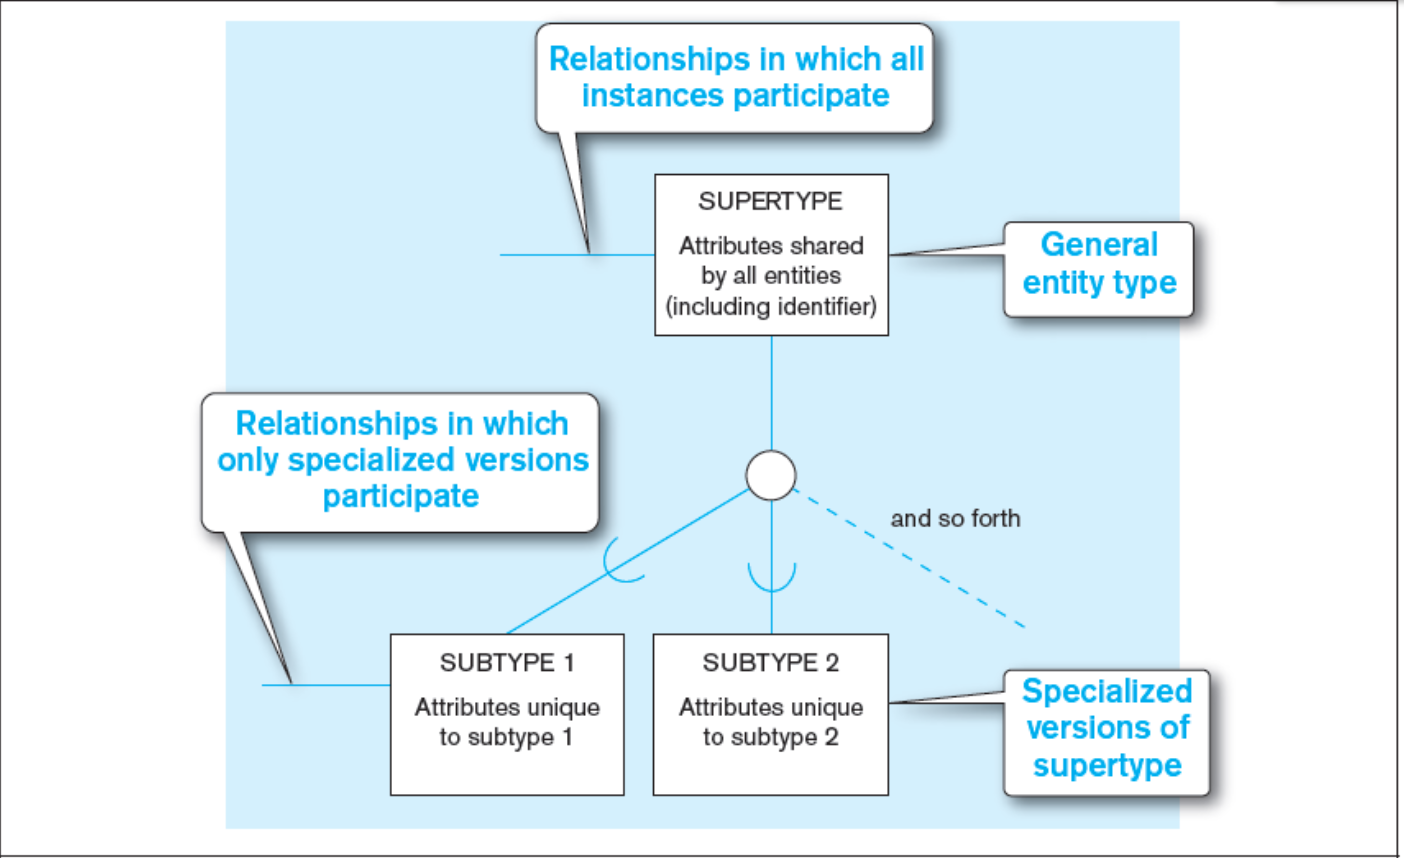
\includegraphics[scale=0.5]{lec3-4}

\subsection{Relationships}

Relationships at the supertype level indicate that all subtypes will participate in the relationship. The instances of a subtype may participate in a relationship unique to that subtype. In this situation, the relationship is shown at the subtype level.\\
\\
\underline{Example of Supertype/subtype relationships in a hospital:}\\
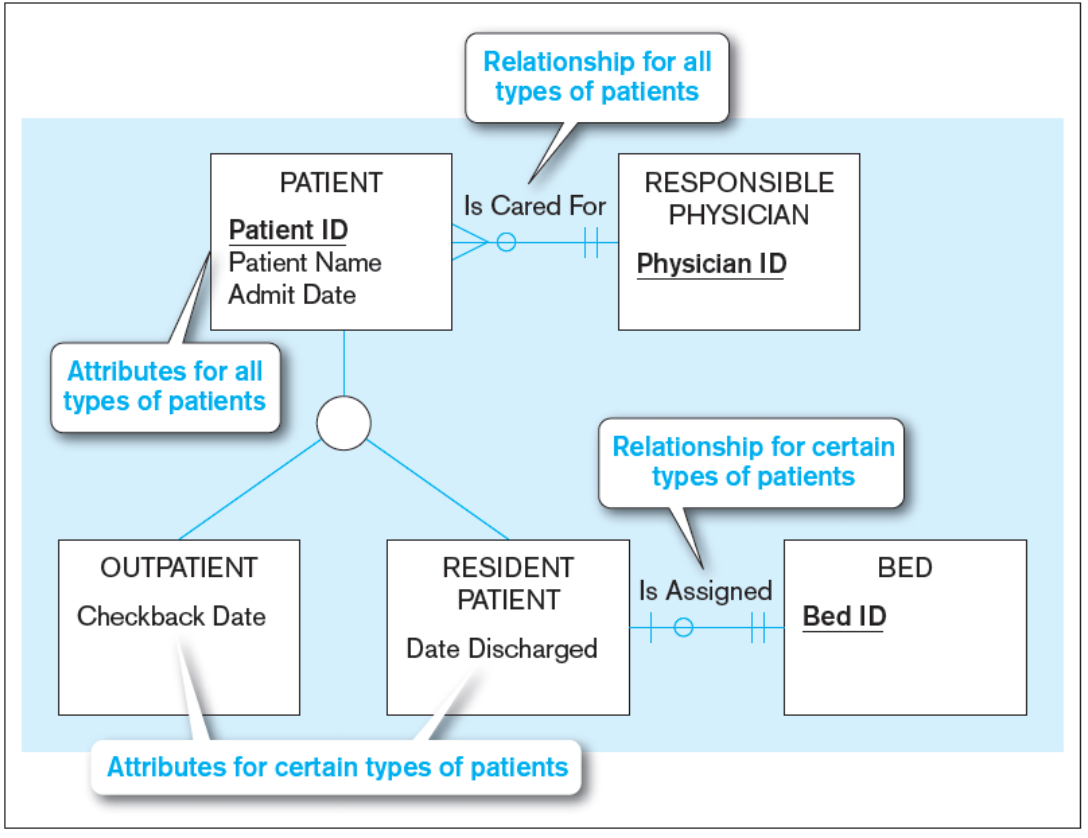
\includegraphics[scale=0.5]{lec3-5}

\subsection{Constraints in Relationship}

\textbf{Completeness Constraints} is whether an instance of a supertype must also be a member of at least one subtype. If yes, then this is a \textbf{total specialization rule} that is denoted by a double line, examples of total specialization include animal types being a specific species, paper publication types, etc. If no, then this is a \textbf{partial specialization rule}, and is denoted by a single line.\\
\\
\textbf{Disjointness Constraints} is whether an instance of a supertype may simultaneously be a member of two (or more) subtypes. If no (that an instance of the supertype can be only one of the subtypes at a time), then it is called the \textbf{Disjoint Rule} and is represented by a $d$, If yes (that an instance of the supertype could be more than one of the subtypes), then it is called the \textbf{Overlap Rule} and is represented by an $o$.\\
\\
\underline{Examples:}\\
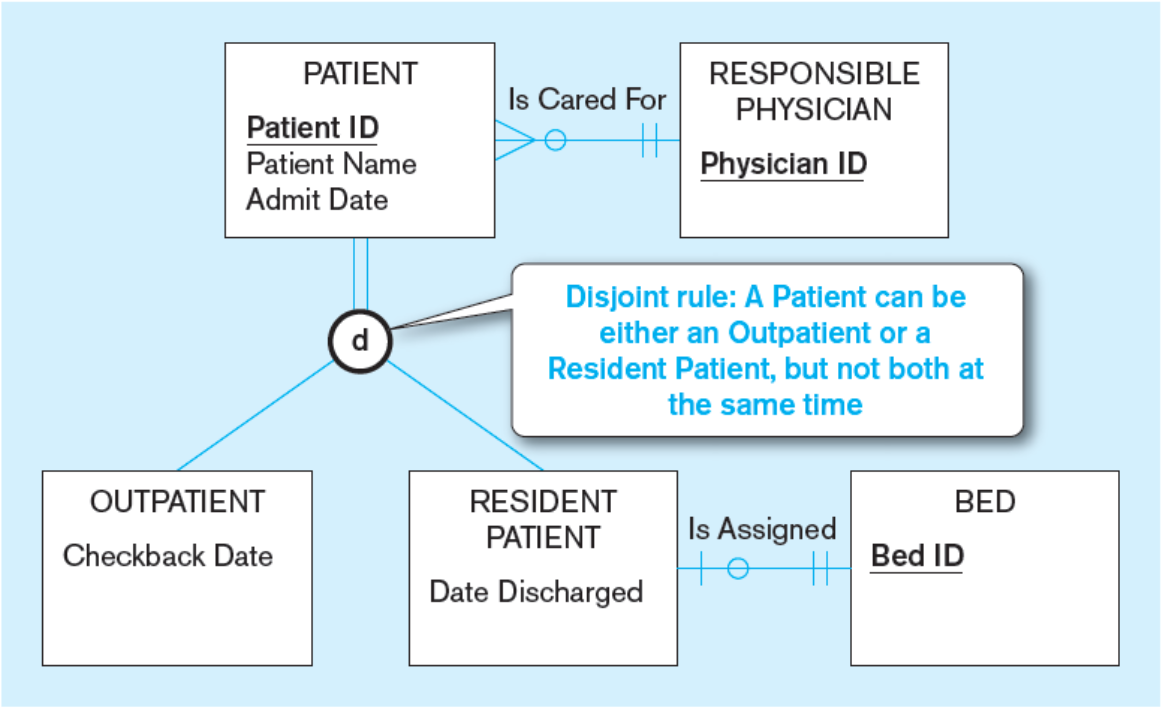
\includegraphics[scale=0.5]{lec3-6}\\
\\
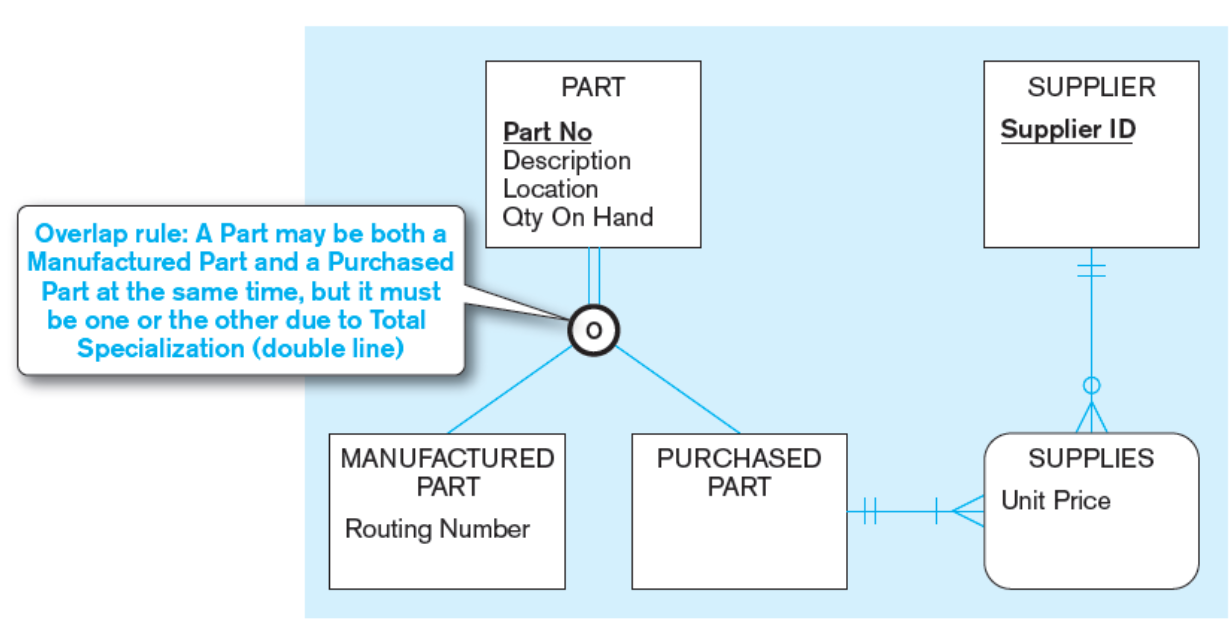
\includegraphics[scale=0.5]{lec3-7}

\subsection{Subtype Discriminator}

An attribute of the subtype whose values determine the target subtype. These subtypes are known as disjoint subtypes.\\
\\
\underline{Example of notation:}\\
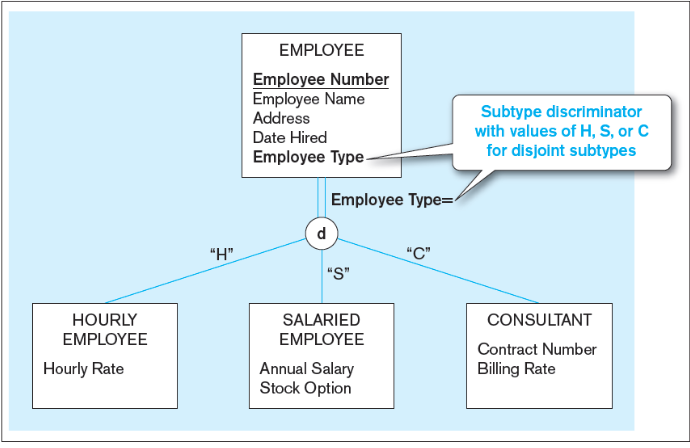
\includegraphics[scale=0.5]{lec3-8}\\

Overlapping also exists for subtype discriminators, it refers to a composite attribute whos subparts pertain to different subtypes. Each subpart contains a boolean value to indicate whether or not the instance belongs to the associated subtype.

\newpage

\section{Thursday, September 28, 2017}

\subsection{Database Design}

\textbf{Database design} is the process of converting EER Models into a relational data model. There are two steps for database design, Logical database design and Physical database design.

\subsection{Relational Data Model}

The relational data model has 3 components, one being the \textbf{Data structure}, such as tables (relations), rows, and columns. Another component being \textbf{Data manipulation}, such as using SQL to retrieve and modify data, and the last being \textbf{Data integrity}, which include mechanisms to implement business rules to maintain integrity of manipulated data.

\subsubsection{Relations}

A relation is a named 2-dimensional table of data, which consists of a set of named columns (attributes / fields) and an arbitrary number of rows (records). An example of short-hand notation of a relation would be (note that the underlined attribute is the identifier attribute): 
$$\text{EMPLOYEE1(\underline{EmpID}}, Name, DeptName, Salary)$$

\underline{Tables as Relations}\\
All relations are tables, but not all tables are relations. The requirements for a table to qualify as a relation are that the table must have a unique name, every attribute must be atomic (not multivalued nor composite), every row must be unique (so there cannot be two rows with the exact same values for all their fields), attributes in tables must have unique names, and the order of the columns and rows must be irrelevant.\\
\\
So in correspondence with the entity-relationship model, Entity Types become Relations, Entity Instances become Rows, and Columns become Attributes.

\begin{tcolorbox}
	\underline{Note:} the word \textbf{relation} in relational database is not the same as the word \textbf{relationship} in the E-R model.
\end{tcolorbox}

\subsubsection{Key Fields}

\paragraph{Primary Key} Primary keys are an attribute or combination of attributes that uniquely identifies each row in a relation. This (These) Primary key(s) must be the same as the identifier in the E-R model and must also be underlined for notation.

\paragraph{Composite Keys} Composite keys are a primary key that consists of more than one attribute.

\paragraph{Foreign Key} A foreign key is an identifier that enables a dependent relationship (on the many side of a relationship) to refer to its parent relation (on the side of the relationship). This foreign key is also no necessarily unique, is denoted by a dashed underlined, and represents a one to many relationship.

\underline{Example:}\\
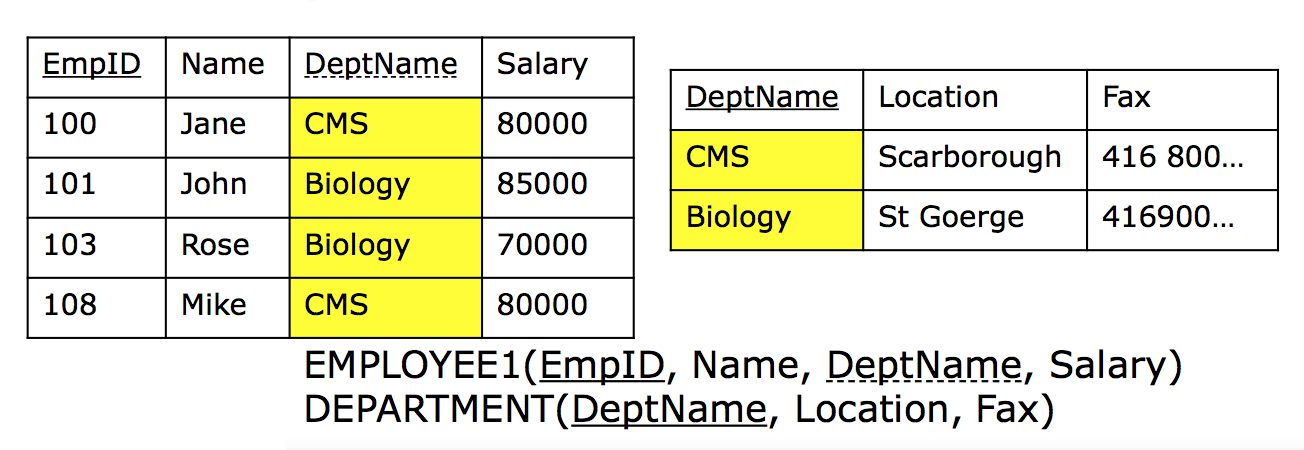
\includegraphics[scale=0.5]{lec4-1}

\subsubsection{Databases}

A Database is a collection of any number of relations, also known as a schema.\\
\\
\underline{Example:}\\
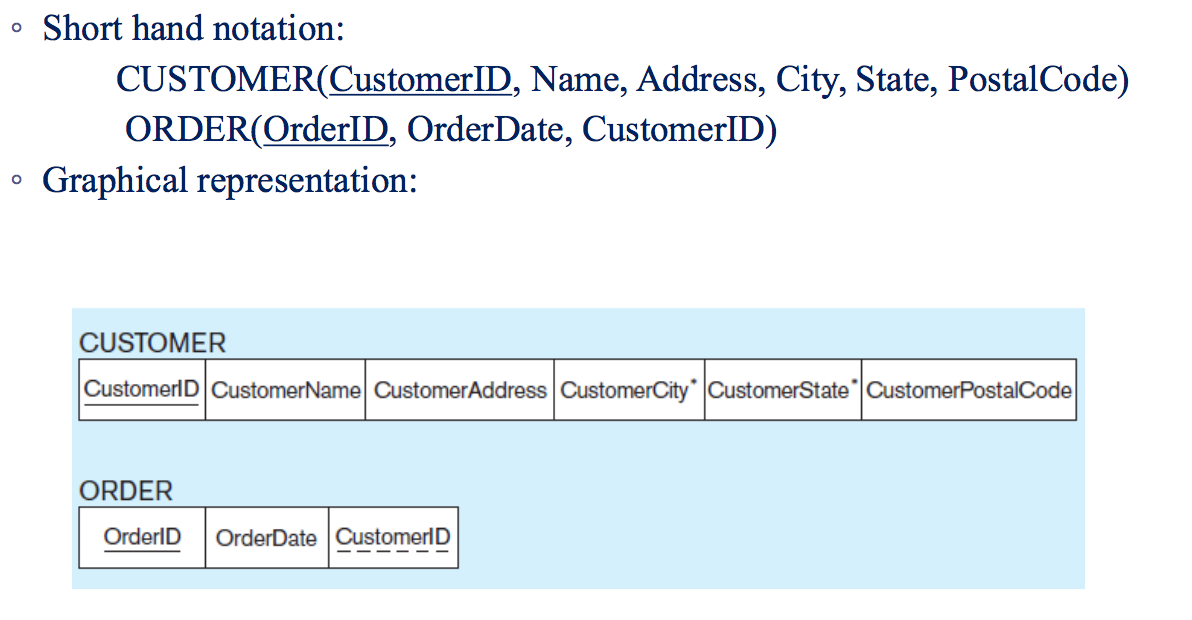
\includegraphics[scale=0.5]{lec4-2}

\subsubsection{Data Integrity}

Data Integrity is another component of a relational data model and more specifically, is the constraints or rules that assures the accuracy and integrity of data in the database. This component includes Domain Constraints, Entity Integrity, and Referential Integrity.

\paragraph{Domain Constraints} A domain constraint is a constraint that states that all values that appear in a column must original from the same domain, including the domain name \slash  data type, size and allowable values or range.
\\
\underline{Example:}\\
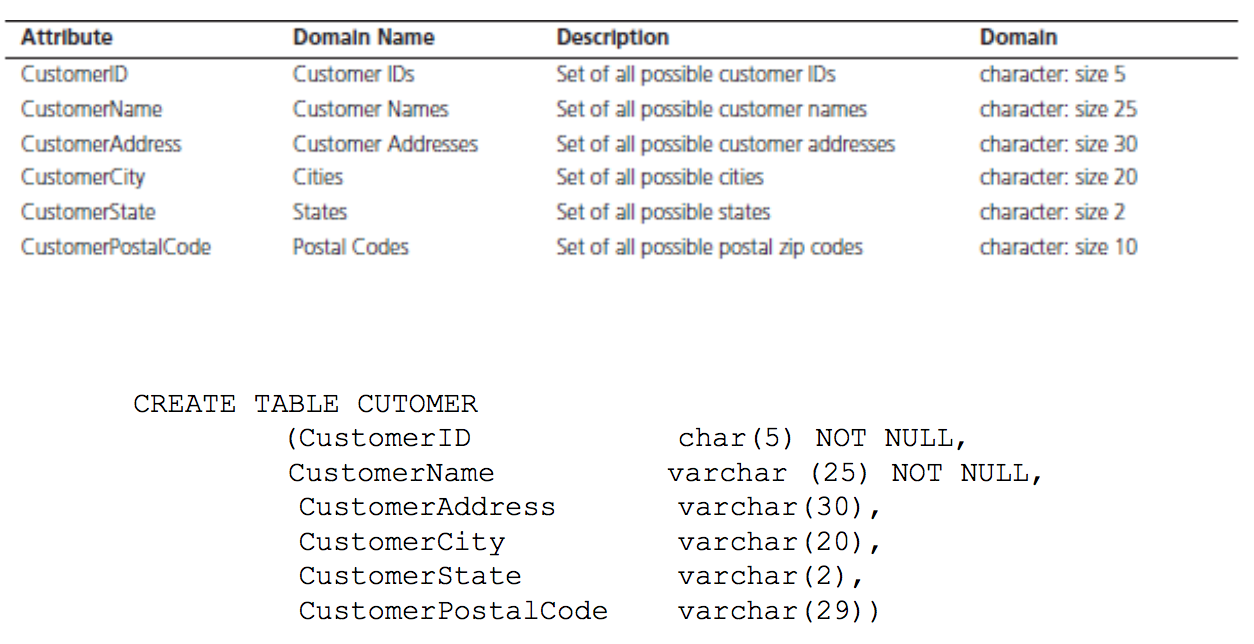
\includegraphics[scale=0.5]{lec4-3}

\paragraph{Entity Integrity} Entity Integrity means that each entity must have a primary key and that the primary key must not be null or nothing.

\paragraph{Referential Integrity} In a one to many relationship, any foreign key value (on the relation of the many side) must match a primary key value in the relation of the one side or the foreign key can be null
\\
\underline{Examples:}\\
\\
A patient may have many prescriptions assigned to them.
$$\text{Patient(\underline{PatientID}}, Name, Address)$$
$$\text{Patient(\underline{PerscriptionID}}, Name, \underline{PatientID})$$

\paragraph{Restrict Delete} When deleting an entity, entities that have other entities referring to them cannot be deleted. Only entities that are not referred to by other entities can be deleted.

\paragraph{Cascade Delete Rule} When deleting an entity, if an entity is referred to by other entities, those other entities will be deleted as well.

\paragraph{Set-to-Null Delete Rule} When deleting an entity, entities that referred to that entity before will now be referring to None.

\subsection{Transforming EER Diagrams into Relations}

Usually the job of transforming EER Diagrams into relations is usually done by the CASE tool, but it is still important to know the transformation process as the CASE tool cannot model complex data relations, such as Ternary and supertype \slash  subtype relations, there are sometimes legitimate alternatives where you will need to choose a particular solution, you must be able to perform quality check on the results obtained from the CASE tool.\\
\\
So for the transformation process, we must do the following:
\begin{enumerate}
	\item{Map Regular Entities}
	\item{Map Weak Entities}
	\item{Map Binary Relations}
	\item{Map Associative Relations}
	\item{Map Unary Relationships}
	\item{Map Ternary (n-ary) Relationships}
	\item{Map Supertype \slash  Subtype Relationships}
\end{enumerate}

\subsubsection{Map Regular Entities}

For Regular Entities, Entity types with simple attributes are made as a basic Relation, with a Relation Name, Relation Attributes and a Relation Primary Key. Entity types with composite attributes have each part of the composite attribute as a Relation attribute, and Entity types with multivalued attributes must create another relation for each multivalued attribute that refers back to the original Relation as the parent.

\subsubsection{Map Weak Entities}

Weak Entities correspond to a normal Relation but with a Surrogate Primary Key and a Foreign Key.

\subsubsection{Mapping Binary Relationships}

\paragraph{one to many} For one to many binary relationships between entities, each element in the many relationship must also have a foreign key corresponding to the ID of the on element.

\paragraph{many to many} For many to many binary relationships between entities, each matching between the two many entity types must have a certificate with two foreign keys in which one refers to one entity type and the other refers to the other entity type. This certificate composite primary key will be the foreign keys.

\paragraph{one to one} For one to one relationships, we let the mandatory relation have a foreign key of the other relation. For mandatory one to one relationships, we can have both relations have foreign keys to the other relation.

\newpage

\section{Thursday, October 5, 2017}

\subsection{Mapping EER into Relations}

\subsubsection{Mapping Associate Entities}

If the identifier is not assigned, associate entities become a relation with foreign keys to its respective parent relations as well as a composite primary key formed from the two foreign keys previously mentioned.\\
\\
If the identifier is assigned, do as before, but the Primary key differs from the foreign keys.

\subsubsection{Mapping Unary Relationships}

For one to one or one to many relationships, the entity is turned into a relation that has a recursive foreign key (the foreign key refers to the primary key of the relation of the same type).\\
\\
For many to many relationships, attributes that come with these relationships are put in a separate component relation with those attributes as well as the two foreign keys for the two sides of the relationship as its composite keys.

\subsubsection{Mapping Ternary (and n-ary) Relationships}

When mapping ternary (and n-ary) relationships, it is simply adding a foreign key in the relation that corresponds to the entity with an optional existence.\\
\\
\underline{Example:}\\
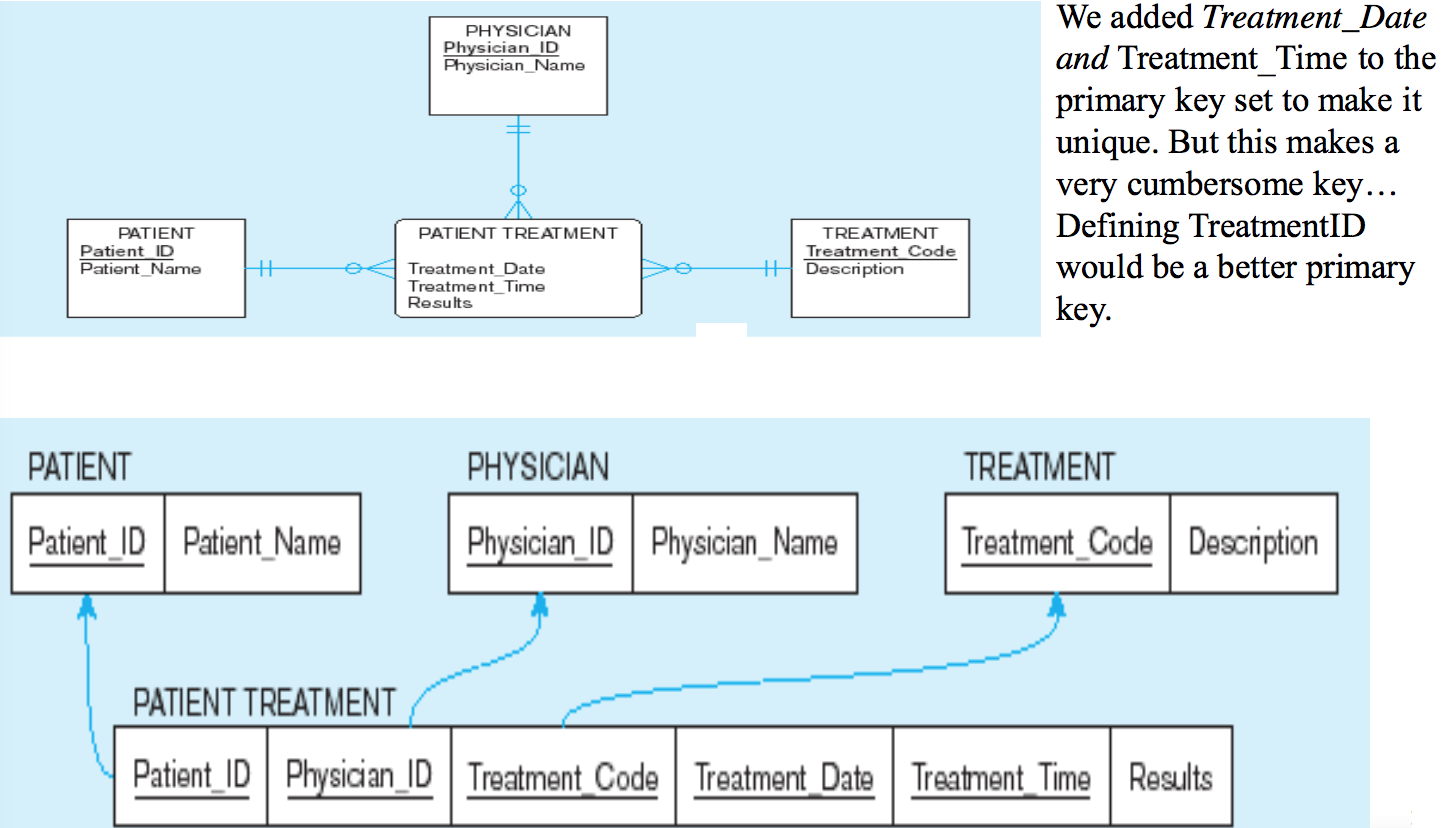
\includegraphics[scale=0.5]{lec5-1}

\subsubsection{Mapping Supertype \slash  Subtype Relationship}

To map these types of relationships, we implement one to one relationships between the subtype and the supertype. So the relations of the subtype must include supertype attributes, a subtype primary key, and a subtype discriminator. The supertype must essentially be a primary table.\\
\\
\underline{Example:}\\
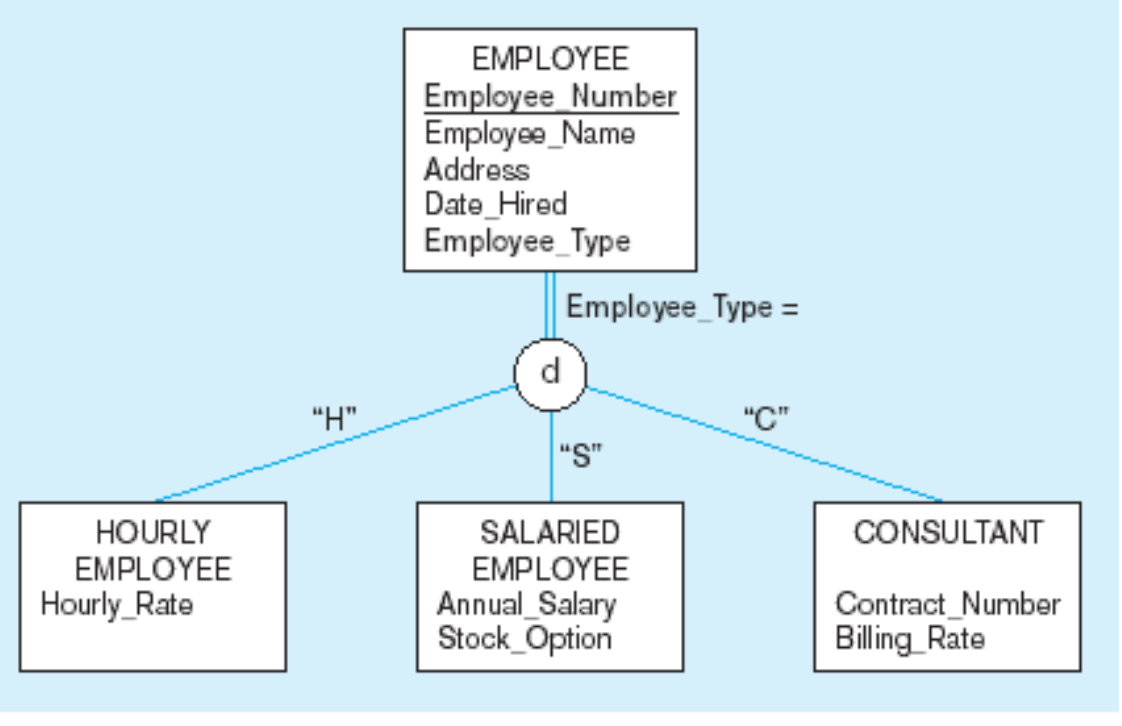
\includegraphics[scale=0.7]{lec5-2}\\
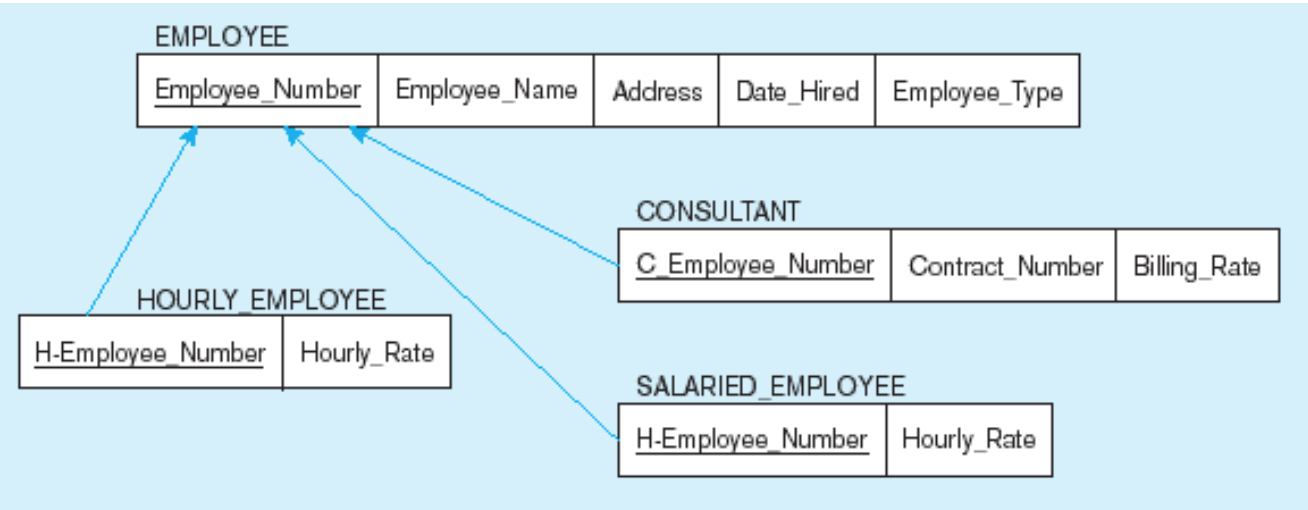
\includegraphics[scale=0.6]{lec5-3}

If the constraint in supertype \slash  subtype followed the overlap rule, we can let the discriminator take on multiple values (for each subtype to have attributes for each discriminator type taking on a boolean stating if that relation is that type of discriminator or not). This can also accommodate the completeness constraint, if it was partial rather than total.

\subsection{Normalization}

There is no guarantee that transforming EER diagrams to relations will remove all the anomalies. \textbf{Normalization} is the process of decomposing relations with anomalies to produce smaller well-structured relations.
\subsubsection{Properties of Well-Structured Relations}
\begin{itemize}
	\item{\textbf{No Data Redundancy}}
	\item{\textbf{No Insertion Anomalies}, which refers to adding new rows to a Table, adding new rows should not force the user to insert some irrelevant data}
	\item{\textbf{No Deletion Anomalies}, which refers to deleting rows and that deleting rows should not cause a loss of data that could be needed for other future rows}
	\item{\textbf{No Modification Anomaly}, which refers to changing data in a row should not force changes to other rows because of duplications}
\end{itemize}

\subsubsection{Steps in Normalization}

\paragraph{First Normal Form (1NF)} The First Normal Form is not allowed to have multivalued attributes, and every attribute value must be atomic. All relations are in the 1st Normal Form, but this does not prevent anomalies from existing.

\paragraph{Functional Dependency} Functional Dependency is when the value of one attribute (the \textbf{determinant}) determines the value of another attribute. Examples include: \textit{CustomerID} being a determinant because it determines the value of the \textit{CustomerName}. Functional Dependency is represented by an arrow, i.e. $A \rightarrow B$

\paragraph{Candidate Keys} A candidate key is a unique identifier, could be an attribute or a combination of attributes that uniquely identifies a row in a relation. One of the candidate keys will become the primary key. Candidate keys are also non-redundant, no attribute in the key can be deleted without destroying the property of unique identification. Note that each non-key field is functionally dependent on every candidate key.\\
\\
Examples include:\\
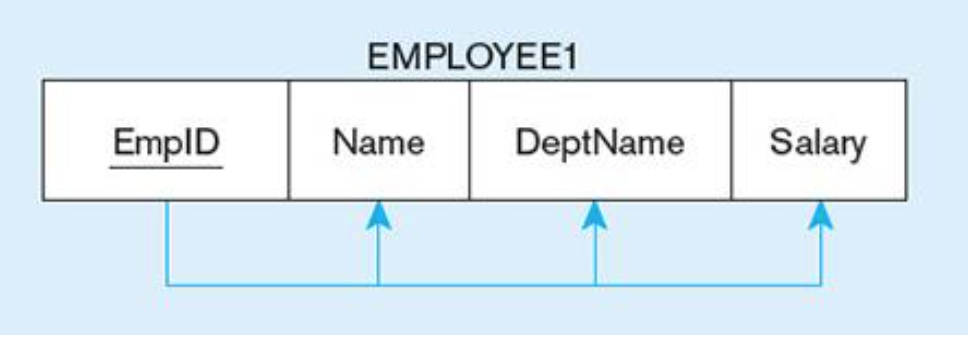
\includegraphics[scale=0.8]{lec5-4}\\
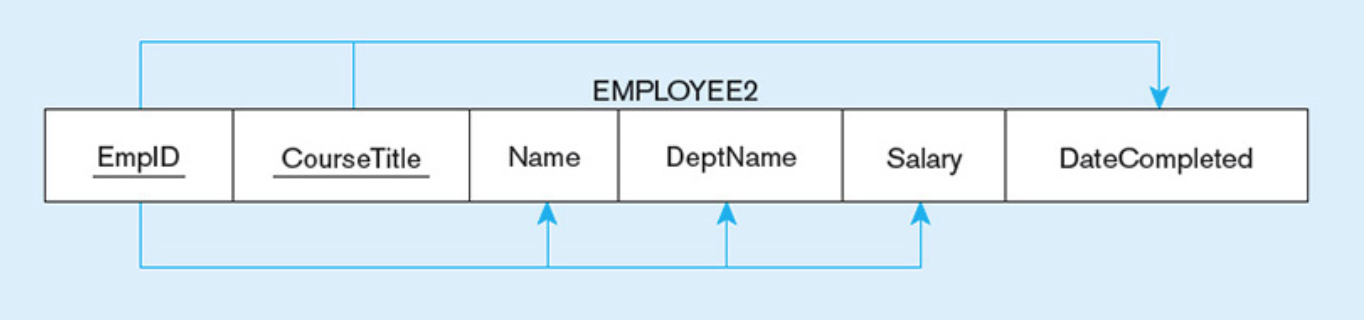
\includegraphics[scale=0.5]{lec5-5}

\newpage

\section{Thursday, October 26, 2017}

\subsection{Normalization (continued)}

\subsubsection{Second Normal Form}

A relation is in Second Normal Form (1Nf) if it is in First Normal Form and there is no partial functional dependency. No partial functional dependency is meant that every non-key attribute is fully functionally dependent of the entire primary key.\\
\\
\underline{Note:} Partial functional dependency is only possible if you have a composite key.\\
\\
\underline{Example of a relation with partial dependencies:}\\
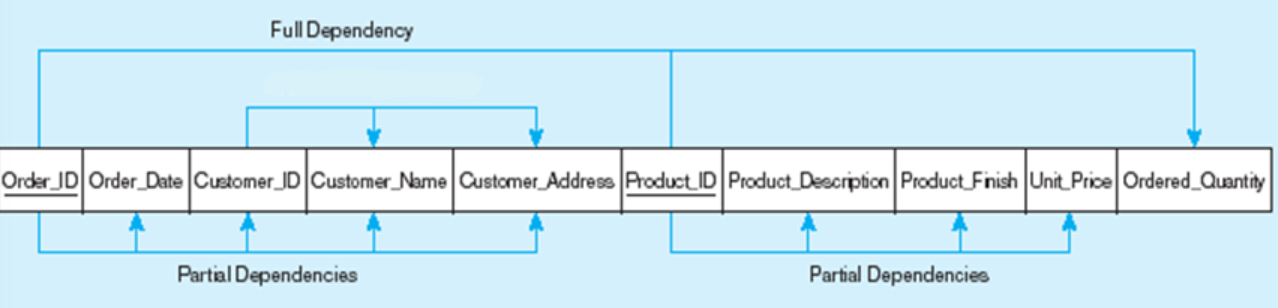
\includegraphics[scale=0.6]{lec6-1}\\
\underline{Example of the same relation, now in 2NF:}\\
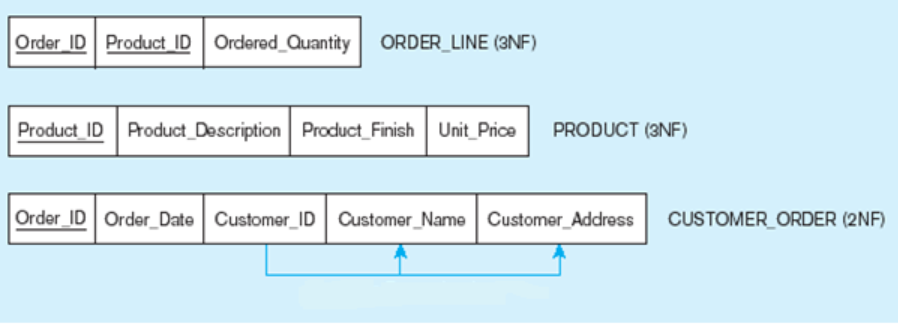
\includegraphics[scale=0.85]{lec6-2}\\
\\
\underline{Another Example of a relation in 1Nf with partial dependencies and the same relations in 2NF:}\\
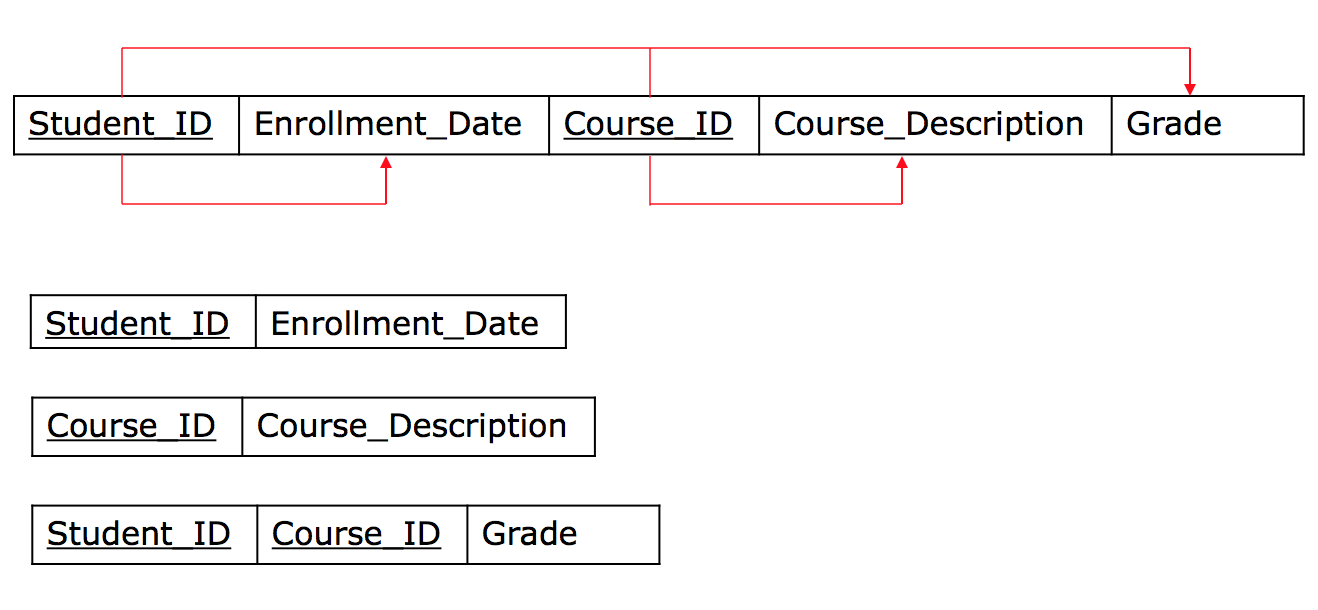
\includegraphics[scale=0.6]{lec6-3}

\subsubsection{Third Normal Form}

A relation is in Third Normal Form (3NF) if the relation is in 2NF and there are no transitive dependencies.\\
\\
\underline{Example of a relation in 2Nf with transitive dependencies and the same relations in 3NF:}\\
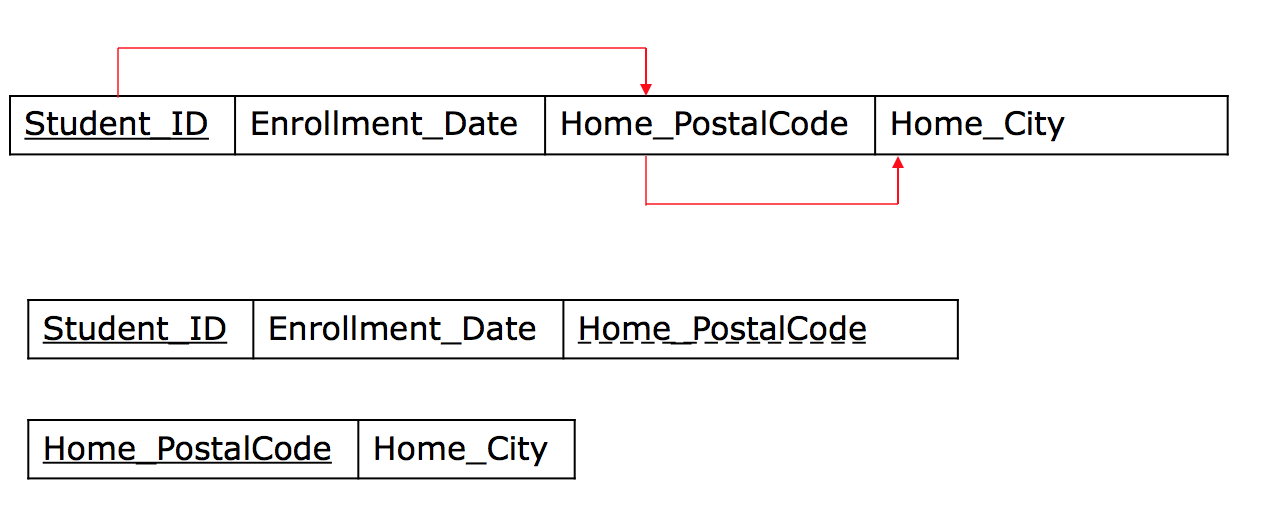
\includegraphics[scale=0.7]{lec6-4}

\subsubsection{Transitive Relations}

Why is a transitive dependency even called that? The formal definition of a transitive relation is $$\forall a,b,c \in X : aRb, bRc \longrightarrow aRc$$
where $X$ is a set and $R$ is a relation

\subsubsection{Boyce-Codd Normal Form}

A relation is in Boyce-Codd Normal Form (NF) if it is both in Third Normal Form and every determinant is a candidate key.\\
\\
\underline{Example of converting a 3NF relation to a Boyce-Codd NF relation:}\\
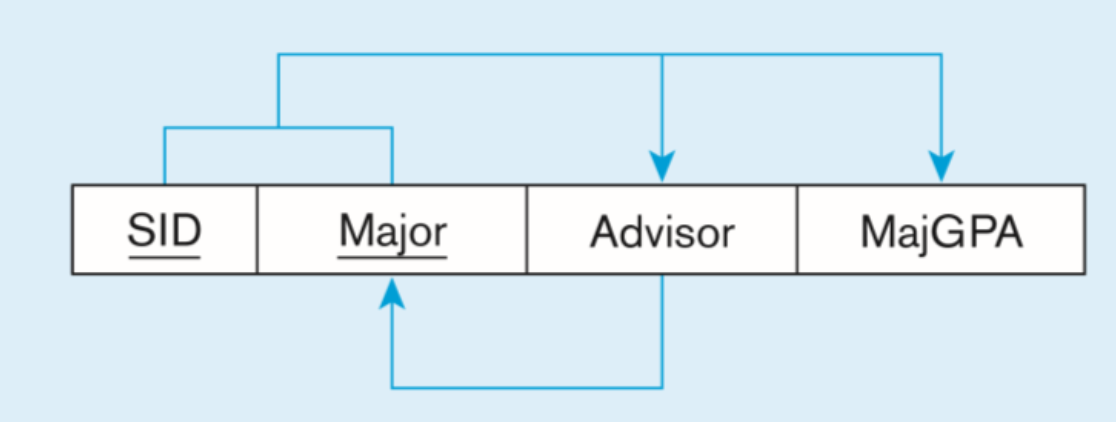
\includegraphics[scale=0.7]{lec6-5}\\
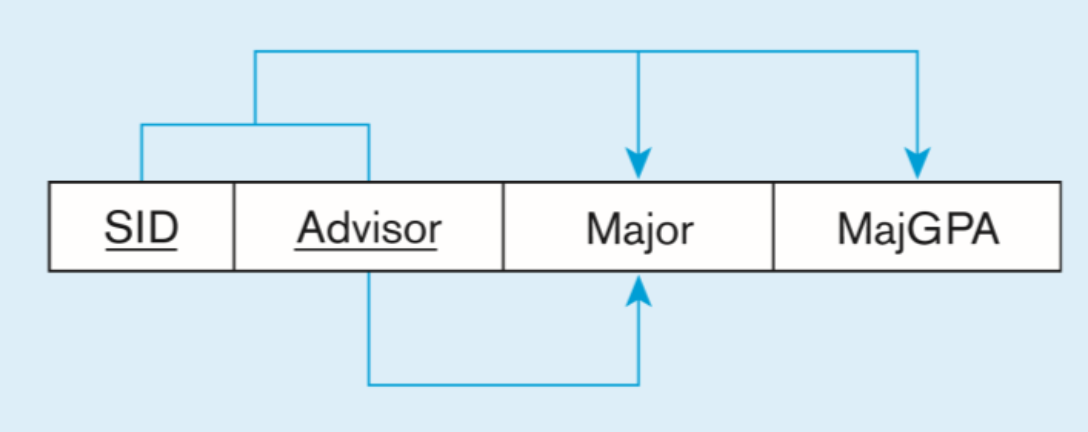
\includegraphics[scale=0.7]{lec6-6}\\
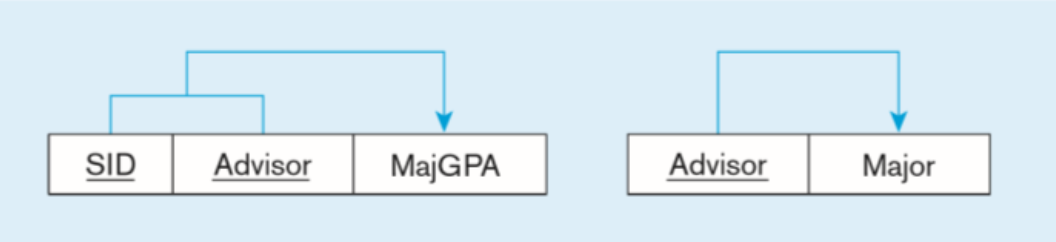
\includegraphics[scale=0.7]{lec6-7}

\subsubsection{Merging Relations}

So there are two ways of creating the structure for your relational databases

\paragraph{Top-Down Analysis} This is when you convert all your business rules into Entity-Relation models which you convert again into Relations. This method requires no merging of relations.

\paragraph{Bottom-Up Analysis} This is when you start out with relations first, and you end up merging relations that are too similar. This happens anyways in large projects where a bunch of sub-teams come together with different relation structures, so they have to be merged together for their work to be merged together.\\
\\
\underline{Example:}\\
\textbf{UnMerged:}\\
EMPLOYEE1(EMPLOYEEID, NAME, ADDRESS, PHONE)\\
EMPLOYEE2(EMPLOYEEID, NAME, ADDRESS, JobCode, NoYears)\\
\\
\textbf{Merged}
EMPLOYEE(EmployeeID, Name, Address, Phone, JobCode, NoYears)
\\
\\
You can also merge relations that differ by a synonym or a homonym:\\
\\
\underline{Example:}\\
\textbf{UnMerged:}\\
STUDENT1 (StudentID, Name, Address)\\
STUDENT2 (MarticulationNo, Name, Address)\\
\\
Assume that STUDENT1's Address refers to their Residing Address while STUDENT2's address refers to their Home Address\\
\\
\textbf{Merged}
STUDENT(StudentID, Name, ResAddress, HomeAddress)
\\
\\
Note how MarticulationNo and StudentID were just two different names for the same attribute and thus, one was removed.\\
\\
You can even merge two relations with transitive dependencies, you just will have to perform normalization to get the relations in 3NF.

\subsubsection{Enterprise Key}

A Primary key is better to be unique across all relations. This key is called an \textit{Enterprise key}

\subsection{Physical Database Design}

The purpose of this is to translate the logical description of data into the technical specifications for storing and retrieving data. This will include more attention on reducing processing time rather than minimizing the space.\\
\\
The Technical Specifications that will be included are designing the fields of and values in our database, this includes data type, coding of values, encryption, and integrity control. Technical Specifics also includes how the database will be indexed, and query optimization.

\subsubsection{Data Types}
Types that are included are specific to the Database Management System, but some common examples include: \textit{Integers, Strings, etc.}

\subsubsection{Coding Technique}

This means that instead of storing the values of each entry in the database, you provide a hash that refers to a lookup table, this may save space but this causes extra lookup time to search this table.

\subsubsection{Controlling Data Integrity}

Database Management Systems support Default values, Range Control, Null Value Control, and Referential Integrity when it comes to managing and maintaining data integrity.

\subsubsection{File Organization}

There are 3 techniques for physically arranging records of a file on secondary storage: \textit{Sequential, Indexed, Hashed}. These techniques are done by the Database Management System itself.

\paragraph{Sequential} Records of the file are stored in sequence by the primary key field values. This is not effective usage and may be only used for database backups only.

\paragraph{Hashed} Records of the file have a key that when put through a hashing algorithm, refers to their relative record number.

\paragraph{Indexed} Records of the file are store either sequentially or nonsequentially and the \textbf{index} is used to locate these records, which can be a table or another data structure that is used to determine the location of requested records in the actual file. This index can either point to a unique record, or another set of records, in which it points to a secondary key index. This technique automatically indexes primary keys.

\subsubsection{Unique and Nonunique Indexes}

\paragraph{Unique (primary) Index} These are typically done for primary keys, but can apply to other unique fields.

\paragraph{NonUnique (secondary) Index} These are done for fields that are often used to group individual entities. (e.g. By zipcode, product category)
\\
\\
\underline{Example of a Index Data Structure:}\\
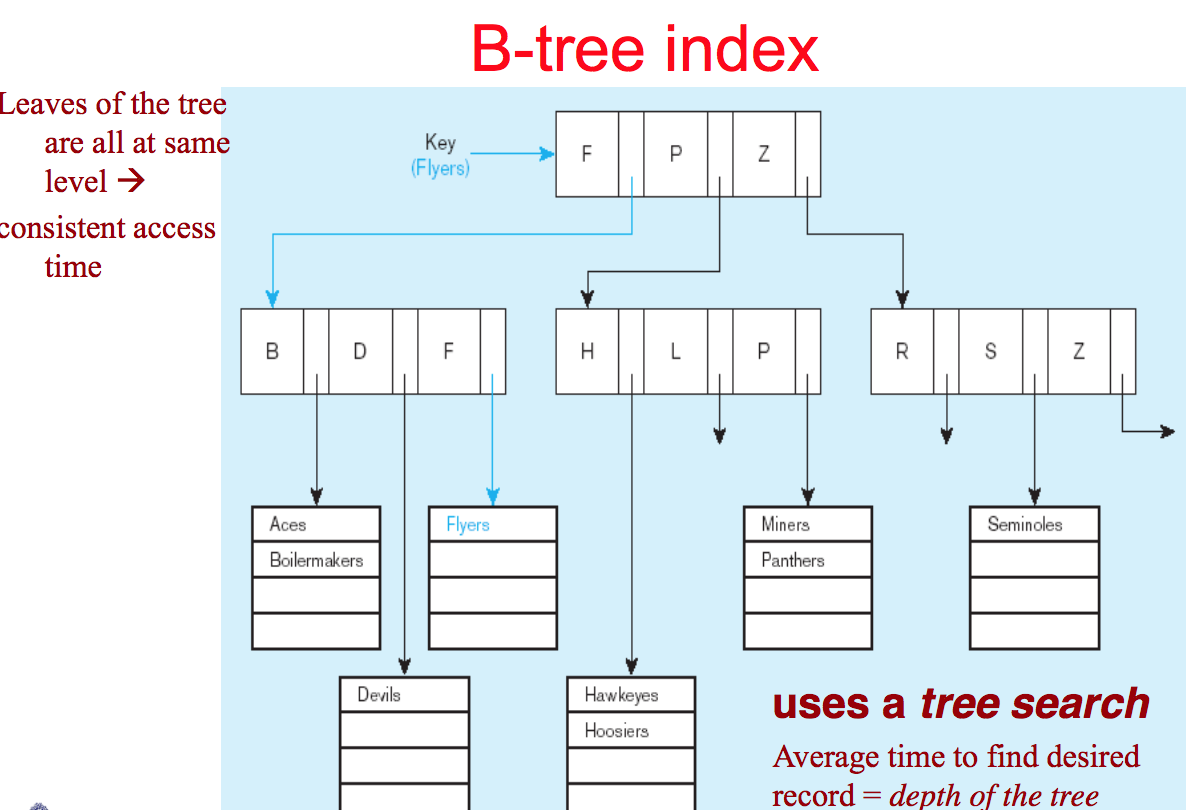
\includegraphics[scale=0.6]{lec6-8}\\

\subsubsection{Rules for Using Indexes}
\begin{enumerate}
	\item{You should use indexing on large tables, preferably when there are more than 100 values but not less than 30 values}
	\item{The indexes should be convenient for frequent searches}
	\item{Avoid use of indexes for fields with long values, it is best to compress the values first}
	\item{Database Management Systems may have a limit on the number of indexes per table and number of bytes per indexed field(s)}
	\item{Be careful of indexing attributes with null values}
\end{enumerate}

\newpage

\section{Thursday, November 2, 2017}

\subsection{SQL}

SQL stands for Structured Query Language, and is the standard for creating and querying relational databases.\\
\\
\paragraph{Relational Database Management System} A database management system that manages data as a collection of tables in which all relationships are represented by common values in related tables

\subsubsection{SQL Environment}

\paragraph{Schema} The structure that contains descriptions of objects created by a user (base tables, views, constraints, domains, character sets, triggers, etc.)
\paragraph{Catalog} A set of schemas that constitute the description of a database
\\
SQL also has 3 types of commands:\\
\paragraph{Data Definition Language (DDL)} These commands are responsible for establishing constraints and creating, altering, and dropping things such as tables, views, and indexes.
\paragraph{Data Manipulation Language (DML)} These commands are responsible for updating, inserting, modifying, and querying a database
\paragraph{Data Control Language (DCL)} These commands are responsible for granting and revoking privilege

\subsubsection{SQL Database Definition}

The following commands fall under DDL. The major CREATE statements that you'll use often are CREATE TABLE, CREATE VIEW, CREATE SCHEMA.

\subsubsection{Table Creation}

\textbf{Steps in Table Creation:}
\begin{enumerate}
	\item{Identify data types for attributes}
	\item{Identify columns that can and cannot be null}
	\item{Identify columns that must be unique (candidate keys)}
	\item{Identify primary key -- foreign key mates}
	\item{Determine the default values for the indexes}
	\item{Identify the constraints on the columns (domain specifications)}
	\item{Create the table associated indexes}
\end{enumerate}

\subsubsection{SQL Example}

The code below is for the following diagram\\
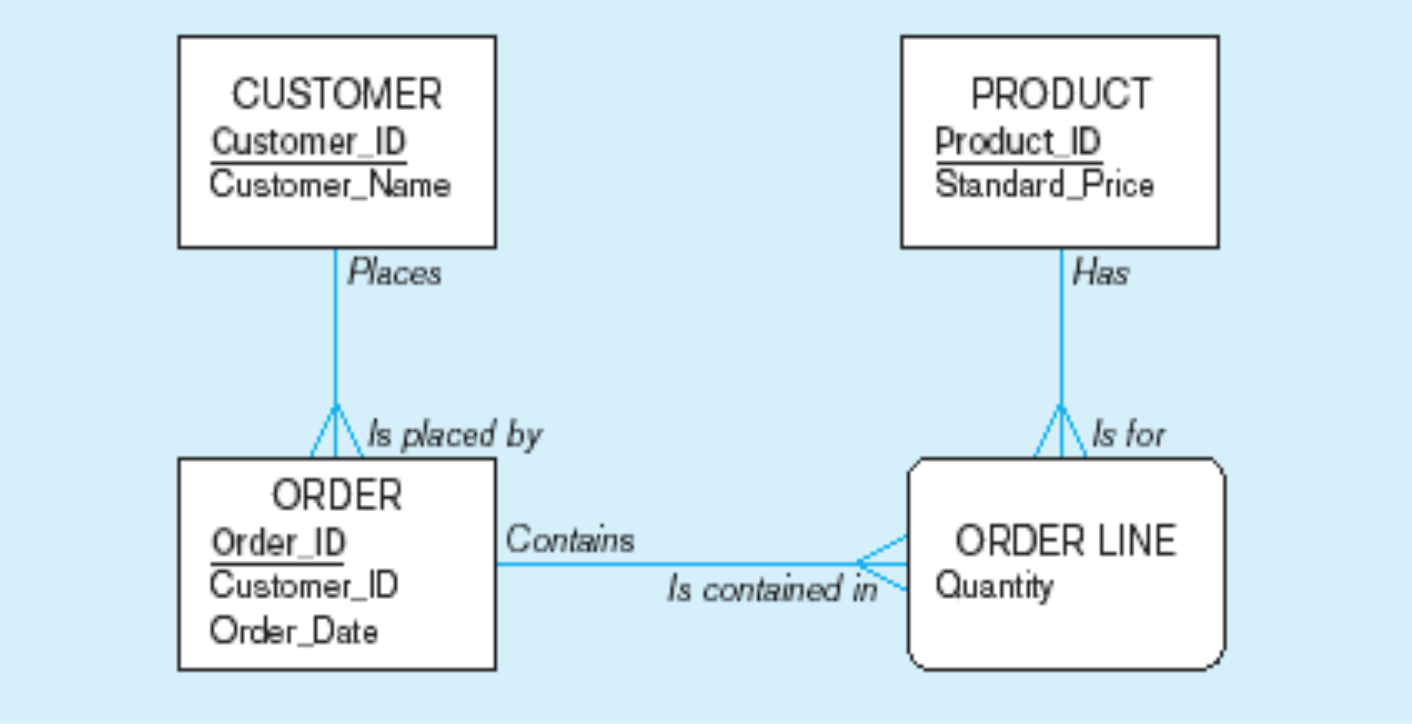
\includegraphics[scale=0.55]{lec7-1}

\begin{lstlisting}[language=SQL]

CREATE TABLE Product_T (
	ProductID Decimal(11,0)NOT NULL, 
	ProductDescription VARCHAR(50), 
	ProductFinish VARCHAR(20)
		CHECK (ProductFinish IN ('Cherry', 'Natural Ash',
		'White Ash', 'Red Oak', 'Natural Oak', 'Walnut')),
	ProductStandardPrice DECIMAL(6,2), 
	ProductLineID INTEGER,
	CONSTRAINT Product_PK PRIMARY KEY (ProductID));

CREATE TABLE OrderLine_T (
	OrderID Decimal(11,0)NOT NULL, 
	ProductID Decimal(11,0)NOT NULL, 
	OrderedQuantity Decimal(11,0),
 	CONSTRAINT OrderLine_PK 
	PRIMARY KEY (OrderID, ProductID),
	CONSTRAINT OrderLine_FK1 
	FOREIGN KEY (OrderID) 
	REFERENCES Order_T(OrderID),
	CONSTRAINT OrderLine_FK2 
	FOREIGN KEY (ProductID) 
	REFERENCES Product_T(ProductID));

CREATE TABLE Customer_T (
	CustomerID Decimal(11,0) not null,
	CustomerName VARCHAR(25) not null, 
	CustomerAddress VARCHAR(25), 
	CustomerCity VARCHAR(20), 
	CustomerState CHAR(2), 
	CustomerPostalCode VARCHAR(9),
	CONSTRAINT Customer_PK PRIMARY KEY (CustomerID));

CREATE TABLE Order_T (
	OrderID Decimal (11,0) not null, 
	OrderDate date,
	CustomerID Decimal(11,0),
	CONSTRAINT Order_PK 
	PRIMARY KEY (OrderID),
  	CONSTRAINT Order_FK 
	FOREIGN KEY (CustomerID) 
	REFERENCES Customer_T(CustomerID));
\end{lstlisting}

\subsubsection{Data Integrity in SQL}

Referential integrity is enforced in SQL as deletes and updates of primary records as well as inserts of dependent records with a null foreign key are null. Delete and Update actions can be specified in SQL, such as:\\

\begin{lstlisting}[language=SQL]
CREATE TABLE Order_T (
	OrderID Decimal (11,0) not null,
	OrderDate date ,
	CustomerID Decimal(11,0),
	CONSTRAINT Order_PK PRIMARY KEY (OrderID), 
	CONSTRAINT Order_FK FOREIGN KEY (CustomerID)
	REFERENCES Customer_T(CustomerID)
	on delete restrict on update cascade);
\end{lstlisting}

\subsubsection{DROP and ALTER}

The DROP command is used to remove Tables, Databases, Schema, and Views from the working session. Altering a table is essentially changing the indexes and data within the table.

\newpage

\section{Thursday, November 9, 2017}

\subsection{SQL (continued)}

\paragraph{Insert Statements} Insert statements adds data to a table

\paragraph{Delete Statements} Delete statements removes rows from a table, it can also be changed to delete certain rows or to just delete all of the rows

\paragraph{Update Statements} Update statements modify data in existing rows

\paragraph{Index} To control processing time and storage efficiency, we need to define indexes on tables. We can create and drop indexes on tables.

\subsubsection{Select Statements}

Select statements are used for queries on single or multiple tables. Here are the clauses of the Select statement:
\begin{itemize}
	\item{\textbf{SELECT}, This is where the list of columns (and expressions) in which the query will return}
	\item{\textbf{FROM}, This is where the table(s) or view(s) are indicated from which the data will be obtained}
	\item{\textbf{WHERE}, Indicate the constraints under which a row must validate in order to be included in the result}
	\item{\textbf{GROUP BY}, This indicates the categorization of the results}
	\item{\textbf{HAVING}, Indicate the conditions under which a category (group) will be included in the result}
	\item{\textbf{ORDER BY}, This is where the specifications on how the result is ordered}
\end{itemize}

Select Statements are processed in the following order:\\
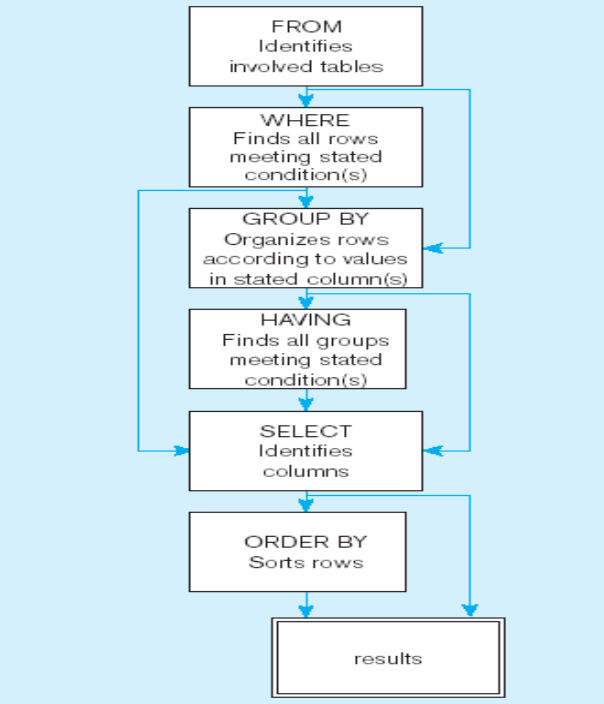
\includegraphics[scale=1]{lec8-1}

\subsubsection{Alias}

An Alias is an alternative column or table name, for example:\\

\begin{lstlisting}[language=SQL]
SELECT P.ProductID AS PROD,
  P.ProductDescription AS DESCR
  FROM Product_T AS P
  WHERE ProductID > 100
  GROUP BY DESCR
  HAVING DESCR = "CHAIR"
  ORDER BY PROD

\end{lstlisting}

In this example, PROD is an alias for P.ProductID and DESCR is an alias for 
P.ProductDescription.

\begin{tcolorbox}
	\underline{Note:} In MySQL, Column Aliases cannot be used in the WHERE clause.
\end{tcolorbox}

\subsubsection{Comparison Operations in SQL}

The following operators are only to be used under the WHERE and HAVING clauses.

\begin{itemize}
	\item{= meaning Equal to}
	\item{$>$  meaning Greater than}
	\item{$>=$ meaning Greater than or equal to}
	\item{$<$  meaning Less than}
	\item{$<=$ meaning Less than or equal to}
	\item{$<>$ or != both mean Not Equal to}
\end{itemize}

\subsubsection{Wildcards, Null, Booleans}

There are 3 wildcards. * which refers to all possibilities. \% which refers to any collection of characters. $\_$ which refers to exactly one character.\\
\\
\underline{Examples:} in the WHERE clause, \% Desk refers to any value with the word "Desk" at the end, "$\_-$drawer" could result in "3-drawer, 4-drawer, etc."\\
\\
For NULL, it is used to refer to values that do not contain anything.

\paragraph{Boolean Operations} Boolean Operators AND, OR, and NOT work as normal.

\subsubsection{ORDER BY Clause and use of IN}

Consider the following example

\begin{lstlisting}[language=SQL]
SELECT CUSTOMER_NAME, CITY, STATE
FROM CUSTOMER_T
  WHERE STATE IN ('FL','TX','CA','HI')
ORDER BY STATE, CUSTOMER_NAME;

\end{lstlisting}

\begin{tcolorbox}
	\underline{Note:} the IN operator is more efficient than separate OR conditions and the default for the ORDER BY clause is ascending.
\end{tcolorbox}

\subsubsection{Aggregate Functions}

Aggregate Functions change what exactly is returned by a SELECT statement, such as

\begin{lstlisting}[language=SQL]
SELECT COUNT(*) FROM ORDER_LINE_V
WHERE ORDER_ID = 1004;

\end{lstlisting}

This is returning the number of data (rows) that satisfy the WHERE clause from "$ORDER\_LINE\_V$".

\begin{tcolorbox}
	\underline{Note:} With aggregate functions, you can't have single-valued columns included in the SELECT clause.
\end{tcolorbox}

\subsubsection{GROUP BY Clause}

For usage with aggregate functions, \textbf{Scalar Aggregate} is a single value returned from a SQL query with an aggregate function and \textbf{Vector Aggregate} is multiple values returned from a SQL query with an aggregate function.

\subsubsection{HAVING}

For use with GROUP BY\\
\\
Example:\\

\begin{lstlisting}[language=SQL]
SELECT CUSTOMER_STATE, COUNT(CUSTOMER_STATE) 
	FROM CUSTOMER_T
	GROUP BY CUSTOMER_STATE
	HAVING COUNT(CUSTOMER_STATE) > 10;

\end{lstlisting}

\subsubsection{Views}
Views provide controlled access to tables. There are also two types of views:
\paragraph{Dynamic View} A "virtual table" created upon request by a user, this table is virtual in the sense that no data is actually sorted, but data from a base table is made available to the user.

\paragraph{Materialized View} A copy or replication of data that is actually stored. This must be refreshed periodically to match the corresponding base tables.

\subsubsection{Check Option}

Check option creates views that are updatable, but trying to update data that is not in the original SELECT statement or that does not satisfy the original SELECT statement will raise an error.

\subsubsection{Advantages and Disadvantages of Views}

Advantages
\begin{itemize}
	\item{You can simplify your query commands with them}
	\item{They assist with data security}
	\item{They enhance programming productivity}
	\item{They maintain concurrency with base table}
	\item{They use little storage space}
	\item{They provide a customized view for the user}
	\item{They establish physical data independence}
\end{itemize}

Disadvantages
\begin{itemize}
	\item{More processing time is used when using a view}
	\item{May not be directly updateable}
\end{itemize}

\newpage
 
\section{Wednesday, November 15, 2017}

I don't remember what was happening exactly, but Marzieh decided to have lecture on Wednesday this week.

\subsection{Relational Algebra}

\subsubsection{Algebra}

An algebra consists of operators and operands, in Arithmetic Algebra, these operations are division, multiplication, addition, etc. and the operands are variables and constants. In Relational Algebra, the operands are different relations and the operations are union, intersection, difference, selection, etc.\\
\\
Queries are our way of referring to relational algebra.

\subsubsection{Relational Algebra Operations}

Assume that $R$ and $S$ are relations and $t$ stands for a tuple:
\begin{enumerate}
	\item{$R \cup S = \{ t : t \in R \vee t \in S  \}$}
	\item{$R \cap S = \{ t : t \in R \wedge t \in S  \}$}
	\item{$R - S = \{ t : t \in R \wedge t \not\in S  \}$}
	\item{
	$\sigma_p (R) = \{ t : t \in R \wedge p \text{ is true}  \}$\\
	Here p is a predicate and the selection operator selects some rows based on the given predicate. For example:
	$$\sigma_{Code =  can} (country) \text{ returns Canadian rows}$$
	}
	\item{
	$\pi_{a_1, ..., a_n} (R) = \{ t[a_1, ... , a_n] : t\in R \}$\\
	Here $a_1, ..., a_n$ are attributes and the projection operator selects the given columns of all rows. For example:
	$$\pi_{name,population} (Country) \text{ returns the name \& populations of the given rows}$$
	}
	\item{$R \times S = \{ (a,b) : a\in R \wedge b \in S \}$\\
	This is just the cartesian product where every row in $R$ is paired with every row in $S$}
	\item{$R \bowtie_c S$\\
	This operation is that the tuples are joined if common attributes are equal (for example, if $R.id = S.id$). $c$ is a condition. There are 2 joins, natural-join and equi-join. Equi-join includes the 2 equal attributes and and natural-join excludes 1 of the 2 equal attributes. }
	\item{
	Outer join: a join that includes all the tuples even the one that does not have a matching value.\\
	Left outer join: $R \leftouterjoin S = (R \bowtie S ) \cup (R - \pi_{a_1,...,a_n} (R \bowtie S) \times \{ null, ... ,null \})$ 
	Right outer join: $R \rightouterjoin S = (R \bowtie S ) \cup (\{ null, ... ,null \} \times (S - \pi_{a_1,...,a_n} (R \bowtie S))$ 
	}
\end{enumerate}

\subsubsection{Self-Join}

For unary relationships. For example, for employees who have supervisors is $$WHERE E.EmployeeSupervisor = M.EmployeeID$$

\subsubsection{Processing Multiple Tables Using Subqueries}

A subquery is placing an inner query (i.e. a SELECT statement) inside an outer query. This can be placed in a condition of the WHERE clause, as a table of the FROM clause or within the HAVING clause.\\
\\
The subqueries can be \textbf{noncorrelated}, which is executed once for the entire outer query, or \textbf{correlated}, which is executed once for each row returned by the other query, this is activated by use the keyword Exist.\\
\\
As an example, the following shows the names of all customers who have placed an order.\\
\begin{lstlisting}[language=SQL]
SELECT CustomerName
	FROM Customer_T
	WHERE CustomerID IN
	(SELECT DISTINCT CustomerID 
	FROM Order_T);

\end{lstlisting}

For processing a noncorrelated subquery, using our example, the subquery (in parentheses) is processed first and an intermediate results table is created. Then the outer query returns the requested customer information for each customer included in the intermediate results table.

\subsubsection{Join vs. Subquery}

Some queries could be accomplished by either a join or a subquery, for example:\\
\\
Join version:
\begin{lstlisting}[language=SQL]
SELECT CustomerName, CustomerAddress, CustomerCity, 
CustomerState, CustomerPostalCode
	FROM Customer_T, Order_T
	WHERE Customer_T.CustomerID = Order_T.CustomerID AND OrderID = 1008;

\end{lstlisting}

Subquery version:
\begin{lstlisting}[language=SQL]
SELECT CustomerName, CustomerAddress, CustomerCity, 
CustomerState, CustomerPostalCode
	FROM Customer_T
	WHERE Customer_T.CustomerID = 
	(SELECT Order_T.CustomerID
		FROM Order_T
		WHERE OrderID = 1008);
\end{lstlisting}

\subsubsection{Correlated Subquery Example}

The following code is for showing all orders that include furniture finished in natural ash.
\begin{lstlisting}[language=SQL]
SELECT DISTINCT OrderID
FROM OrderLine_T
WHERE EXISTS
	(SELECT *
	FROM Product_T
	WHERE ProductID = OrderLine_T.ProductID
	AND Productfinish = 'Natural Ash');
\end{lstlisting}

The EXISTS operator returns either TRUE or FALSE. A correlated subquery always refers to an attribute from a table referenced in the outer query. In this example, it is the line:

\begin{lstlisting}[language=SQL]
	WHERE ProductID = OrderLine_T.ProductID
\end{lstlisting}

\subsubsection{Derived Table Subquery Example}

The following query shows all products whose standard price is higher than the average price:

\begin{lstlisting}[language=SQL]
SELECT ProductDescription, ProductStandardPrice, AvgPrice
	FROM 
	(SELECT AVG(ProductStandardPrice) AvgPrice FROM Product_T),
	Product_T
	WHERE ProductStandardPrice > AvgPrice;
\end{lstlisting}

The WHERE clause normal cannot include aggregate functions but because the aggregate is performed in the subquery, its results can be used in the outer query's WHERE clause.

\subsubsection{Union Queries}

Union queries is essentially combining the output (union of multiple queries) together into a single result table.

\begin{tcolorbox}
	\underline{Note:} With UNION queries, the quantity and data types of the attributes in the select clauses of both queries must be identical.
\end{tcolorbox}

\begin{lstlisting}[language=SQL]
SELECT C1.CustomerID, CustomerName, OrderedQuality, 
'Largest Quantity' AS QUANTITY
FROM Customer_T C1, Order_T O1, OrderLine_T Q1
	WHERE C1.CustomerID = O1.CustomerID
	AND O1.OrderID = Q1.OrderID
	AND OrderedQuantity =
	(SELECT MAX(Ordered Quantity)
	FROM OrderLine_T)
UNION
SELECT C1.CustomerID, CustomerName, OrderedQuality, 
'Smallest Quantity' AS QUANTITY
FROM Customer_T C1, Order_T O1, OrderLine_T Q1
	WHERE C1.CustomerID = O1.CustomerID
	AND O1.OrderID = Q1.OrderID
	AND OrderedQuantity =
	(SELECT MIN(Ordered Quantity)
	FROM OrderLine_T)
ORDER BY 3;
\end{lstlisting}

\subsubsection{Conditional Expressions Using Case Keyword}

This is a feature that is available with newer versions of SQL. Keyword COALESCE returns the first non-null expression among its arguments, and keyword NULLIF returns null if the two specified expressions are equal and returns the first expression if they aren't.\\
\\
Usage for NULLIF and COALESCE:
\begin{lstlisting}[language=SQL]
NULLIF(expression, expression)
COALESCE(expression, ... , expression)
\end{lstlisting}

\begin{tcolorbox}
	\underline{Note:} COALESCE can take one or multiple expressions.
\end{tcolorbox}

Example of the CASE usage:\\
\begin{lstlisting}[language=SQL]
SELECT CASE
	WHEN ProductLine = 1 THEN ProductDescription
	ELSE '####'
END AS ProductDescription
FROM Product_T;
\end{lstlisting}

Another CASE example:\\
\begin{lstlisting}[language=SQL]
SELECT ProductNumber, Category =
	CASE ProductLine
		WHEN 'R' THEN 'Road'
		WHEN 'M' THEN 'Mountain'
		WHEN 'T' THEN 'Touring'
		WHEN 'S' THEN 'Other sale items'
		ELSE 'Not for sale'
	END,
	Name
FROM Production.Product
ORDER BY ProductNumber;
\end{lstlisting}

A Coalesce example:\\
\begin{lstlisting}[language=SQL]
SELECT Name, Class, Color, ProductNumber,
	COALESCE(Class, Color, ProductNumber) AS
	FirstNotNull
FROM Production.Product;
\end{lstlisting}

Here are two SELECT statements of NULLIF and CASE usage that do the same thing:\\
\\
NULLIF:
\begin{lstlisting}[language=SQL]
SELECT ProductID, MakeFlag, FinishedGoodsFlag,
	NULLIF(MakeFlag, FinishedGoodsFlag) AS 'Null if Equal'
FROM Production.Product
WHERE ProductID < 10;
\end{lstlisting}

CASE:
\begin{lstlisting}[language=SQL]
SELECT ProductID, MakeFlag, FinishedGoodsFlag,
	'Null if Equal' = CASE
	WHEN MakeFlag =. FinishedGoodsFlag THEN NULL
	ELSE MakeFlag
	END
FROM Production.Product
WHERE ProductID < 10;
\end{lstlisting}

\newpage

\section{Thursday, November 23, 2017}

\subsection{Transaction}

A transaction is a set of commands that is atomic, discrete in a sense where it is either done or not. To ensure transaction integrity, BEGIN TRANSACTION marks the beginning of a transaction, COMMIT makes all updates permanent and ROLLBACK cancels updates since the last commit.\\
\\
So when \textit{valid} information is inserted, the work is committed and all the chances to the data will be made permanent. However, when \textit{invalid} information is inserted, the transaction will be cancelled and all changes made will be rolled back to before the transaction began.

\subsection{Routines and Triggers}

\paragraph{Routines} are program modules that execute when called. They can be \textbf{Functions}, \textbf{Procedures}, and \textbf{Triggers}. Triggers being routines that execute in a response to a database event (when the database management system inserts, updates or deletes). These routines are stored in the database and are controlled by the Database Management System. They are good for preserving data integrity, data auditing and security.\\
\\
The differences between routines and triggers are that routines are called directly and perform a routine or return a value, and triggers are implicitly called in the event of a database event and performs a trigger action.

\subsubsection{Trigger Syntax in MySQL}

\begin{lstlisting}[language=SQL]
CREATE TRIGGER trigger_name
	{BEFORE | AFTER}
	{INSERT | UPDATE | DELETE}
	ON table_name
	FOR EACH ROW trigger_body
\end{lstlisting}

\subsubsection{Routines Syntax in MySQL}

\begin{lstlisting}[language=SQL]
CREATE PROCEDURE sp_name([procedure_parameter[,...]])
	routine_body
CREATE FUNCTION sp_name ([function_parameter[,...]]) RETURNS type
	routine_body
\end{lstlisting}

Looking at the syntax here:\\
The \textbf{procedure parameter} can either be IN, OUT, or INOUT, also has a parameter name and a type.\\
\\
The \textbf{function parameter} has a name and a type\\
\\
The different \textbf{types} are any valid MySQL data type.\\
\\
The \textbf{routine body} is just a valid SQL routine statement.

\subsubsection{More Complicated SQL Queries}

As Production Databases could contain thousands of tables and tables contain hundreds of columns, writing single queries may not be feasible, so we sometimes combine queries, by using subqueries and creating views.

\subsubsection{Example of a Query using a View}

\begin{lstlisting}[language=SQL]
CREATE View TSales AS
SELECT SalespersonName,
	ProductDescription,
	SUM(OrderedQuantity) AS Totorders
FROM Salesperson_T, OrderLine_T, Product_T, Order_T
	WHERE Salesperson_T.SalespersonID=Order_T.SalespersonID
	AND Order_T.OrderID = OrderLine_T.OrderID
	AND OrderLine_T.ProductID=Product_T.ProductID
	GROUP BY SalespersonName, ProductDescription;
	
SELECT SalespersonName, ProductDescription
	FROM TSales AS A
	WHERE Totorders = (SELECT MAX(Totorders) FROM TSales B
	WHERE B.SalespersonName=A.SalespersonName);
\end{lstlisting}

\subsubsection{Tips For Developing Efficient Queries}

\begin{itemize}
	\item{Be familiar with the data model}
	\item{Understand the desired results of the query}
	\item{Know the attributes desired in the query}
	\item{Identify the entities that contain desired attributes}
	\item{Construct a WHERE equality for each link}
	\item{Fine tune with GROUP BY, HAVING, DISTINCT, NOT IN clauses if needed}
	\item{Consider the effect on unusual data, such as null values when computing AVG and SUM.}
	\item{Avoid using SELECT $*$ for tables with many columns}
	\item{Avoid subqueries if possible, instead write a single query. More specifically, correlated subqueries}
	\item{If data is used many times, consider making a separate query and storing it as a view.}
	\item{Understand how indexes are used in query processing. For example, equality operations in the WHERE clause use indexes, while using inequality operations (NOT IN) in the WHERE clause does not}
	\item{Break complex queries into multiple simple parts}
	\item{Do not combine a query with itself (if possible, avoid self-joins)}
	\item{Create temporary tables (materialized views) for groups of queries}
	\item{Combine update operations}
	\item{Retrieve only the data you need}
	\item{Don't have the Database Management System sort without an index}
	\item{Learn how to track query processing time}
	\item{Learn to review query plans with the EXPLAIN command}
	\item{Consider the total query processing time for ad hoc queries}
\end{itemize}

\subsection{SQL}

\paragraph{Interactive SQL:} What we have done up to know

\paragraph{Embedded SQL:} Including hard-coded SQL statements in a program written in another language such as C or Java.

\paragraph{Dynamic SQL:} Ability for an application program to generate SQL code on the fly, as the application is running

\subsubsection{Reasons to Embed SQL}

\begin{itemize}
	\item{Can create a more flexible, accessible interface for the user}
	\item{Possible performance improvement}
	\item{Database security improvement; Grants access only to the application instead of the user.}
\end{itemize}

\newpage

\section{Thursday, November 30, 2017}

\subsection{SQL Injection Attacks (SQLi)}

SQL Injections are one of the most dangerous and common network-based security threats. It's essentially sending malicious code to a database server directly, where the Database runs the malicious code as legitimate code, so the data that was supposed to be safe and secure is accessible publicly.\\
\\
So SQL Injections works on the dynamic component of an application, and allows an intruder to Delete and modify data, Run OS commands, and create a DOS (Denial of Service) attack.

\subsubsection{How it works}

The attack is essentially about taking advantage of a text field that translates into a WHERE clause of a database, you would have to write a tautology (which is a condition that always evaluates to true) to access all the information from the tables that the WHERE clause relates to. It also involves black box testing to check how the text in the text field is parsed, and from there, we can find out how a database is stored.

\subsubsection{SQL Injection Attack Countermeasure}

Ways to defend against a SQL Injection is to sanitize the input to remove malicious input or render it useless, white list input validation, use of parameterized queries, and use of stored procedures.

\end{document}








































